\documentclass[12pt, a4paper,
%oneside,      %% -- odkomentujte, pokud chcete svou práci mít pouze jednostrannou, mezera pro hřbet pak automaticky bude pouze na levé straně
%twoside,        %% -- pro oboustranné práce, mezera pro hřbet následně střídá strany.
openright
]{report}

%% Nutné balíčky a nastavení
%%%%%%%%%%%%%%%%%%%%%%%%%%%%

%% Proměnné
\newcommand\obor{INFORMAČNÍ TECHNOLOGIE} %% -- napiš číslo a název tvého oboru
\newcommand\kodOboru{18-20-M/01} %% -- napiš číslo a název tvého oboru
\newcommand\zamereni{se zaměřením na počítačové sítě a programování} %% -- napiš číslo a název tvého oboru
\newcommand\skola{Střední škola průmyslová a umělecká, Opava} %% vyplň název školy
\newcommand\trida{IT4} %% vyplň jméno svého konzultanta
\newcommand\jmenoAutora{Matěj Kotrba}  %% vyplň své jméno
\newcommand\skolniRok{2023/24} %% vyplň rok
\newcommand\datumOdevzdani{1. 1. 2024} %% vyplň rok
\newcommand\nazevPrace{Effio - webová aplikace pro vytváření testů} %% vyplň název své práce

\title{\nazevPrace} %% -- Název tvé práce
\author{\jmenoAutora} %% -- tvé jméno
\date{\datumOdevzdani} %% -- rok, kdy píšeš SOČku

\usepackage[top=2.5cm, bottom=2.5cm, left=3.5cm, right=1.5cm]{geometry} %% nastaví okraje, left -- vnitřní okraj, right -- vnější okraj

\usepackage[czech]{babel} %% balík babel pro sazbu v češtině
\usepackage[utf8]{inputenc} %% balíky pro kódování textu
\usepackage[T1]{fontenc}
\usepackage{cmap} %% balíček zajišťující, že vytvořené PDF bude prohledávatelné a kopírovatelné
\usepackage{indentfirst}

\usepackage{graphicx} %% balík pro vkládání obrázků

\usepackage{subcaption} %% balíček pro vkládání podobrázků

\usepackage{hyperref} %% balíček, který v PDF vytváří odkazy

\usepackage{enumitem}

\linespread{1.25} %% řádkování
\setlength{\parskip}{0.5em} %% odsazení mezi odstavci


\usepackage[pagestyles]{titlesec} %% balíček pro úpravu stylu kapitol a sekcí
\titleformat{\chapter}[block]{\scshape\bfseries\LARGE}{\thechapter}{10pt}{\vspace{0pt}}[\vspace{-22pt}]
\titleformat{\section}[block]{\scshape\bfseries\Large}{\thesection}{10pt}{\vspace{0pt}}
\titleformat{\subsection}[block]{\bfseries\large}{\thesubsection}{10pt}{\vspace{0pt}}


\usepackage{tocloft} % Balíček umožní přizpůsobit vzhled tabulky obsahu
\setlength{\cftbeforechapskip}{0pt}  % Menší rozestup pro kapitoly
\setlength{\cftbeforesecskip}{0pt}   % Menší rozestup pro sekce

\setcounter{secnumdepth}{2}
\setcounter{tocdepth}{1}
\usepackage{fancyhdr}
\pagestyle{fancy}
\fancyhf{}
\renewcommand{\headrulewidth}{0pt}
\fancyfoot[C]{\thepage}

\usepackage{booktabs}

\usepackage{url}

%% Balíčky co se můžou hodit :) 
%%%%%%%%%%%%%%%%%%%%%%%%%%%%%%%

\usepackage{pdfpages} %% Balíček umožňující vkládat stránky z PDF souborů, 

\usepackage{upgreek} %% Balíček pro sazbu stojatých řeckých písmen, třeba u jednotky mikrometr. Například stojaté mí: \upmu, stojaté pí: \uppi

\usepackage{amsmath}    %% Balíčky amsmath a amsfonts 
\usepackage{amsfonts}   %% pro sazbu matematických symbolů
\usepackage{esint}     %% pro sazbu různých integrálů (např \oiint)
\usepackage{mathrsfs}
\usepackage{helvet} % Helvet font
\usepackage{mathptmx} % Times New Roman
\usepackage{Oswald} % Oswald font
\usepackage{float}

%% makra pro sazbu matematiky
\newcommand{\dif}{\mathrm{d}} %% makro pro sazbu diferenciálu, místo toho
%% abych musel psát '\mathrm{d}' mi stačí napsat '\dif' což je mnohem 
%% kratší a mohu si tak usnadnit práci

\let\oldchapter\chapter
\renewcommand{\chapter}{
	\clearpage
	\pagestyle{fancy}
	\oldchapter
}

\usepackage{listings}
\usepackage{xcolor}

\renewcommand{\lstlistingname}{Kód}% Listing -> Algorithm
\renewcommand{\lstlistlistingname}{Seznam programových kódů}% List of Listings -> List of Algorithms

%% Definice 
\lstdefinelanguage{JavaScript}{
	morekeywords=[1]{break, continue, delete, else, for, function, if, in,
		new, return, this, typeof, var, void, while, with},
	% Literals, primitive types, and reference types.
	morekeywords=[2]{false, null, true, boolean, number, undefined,
		Array, Boolean, Date, Math, Number, String, Object},
	% Built-ins.
	morekeywords=[3]{eval, parseInt, parseFloat, escape, unescape},
	sensitive,
	morecomment=[s]{/*}{*/},
	morecomment=[l]//,
	morecomment=[s]{/**}{*/}, % JavaDoc style comments
	morestring=[b]',
	morestring=[b]"
}[keywords, comments, strings]


\lstdefinelanguage[ECMAScript2015]{JavaScript}[]{JavaScript}{
	morekeywords=[1]{await, async, case, catch, class, const, default, do,
		enum, export, extends, finally, from, implements, import, instanceof,
		let, static, super, switch, throw, try},
	morestring=[b]` % Interpolation strings.
}

\lstalias[]{ES6}[ECMAScript2015]{JavaScript}

% Nastavení barev
% Requires package: color.
\definecolor{mediumgray}{rgb}{0.3, 0.4, 0.4}
\definecolor{mediumblue}{rgb}{0.0, 0.0, 0.8}
\definecolor{forestgreen}{rgb}{0.13, 0.55, 0.13}
\definecolor{darkviolet}{rgb}{0.58, 0.0, 0.83}
\definecolor{royalblue}{rgb}{0.25, 0.41, 0.88}
\definecolor{crimson}{rgb}{0.86, 0.8, 0.24}


\lstdefinestyle{JSES6Base}{
	backgroundcolor=\color{white},
	basicstyle=\ttfamily\footnotesize,
	breakatwhitespace=false,
	breaklines=true,
	captionpos=b,
	columns=fullflexible,
	commentstyle=\color{mediumgray}\upshape,
	emph={},
	emphstyle=\color{crimson},
	extendedchars=true,  % requires inputenc
	fontadjust=true,
	frame=single,
	identifierstyle=\color{black},
	keepspaces=true,
	keywordstyle=\color{mediumblue},
	keywordstyle={[2]\color{darkviolet}},
	keywordstyle={[3]\color{royalblue}},
 literate=%
{á}{{\'a}}1 {č}{{\v{c}}}1 {ď}{{\v{d}}}1 {é}{{\'e}}1 {ě}{{\v{e}}}1
{í}{{\'i}}1 {ň}{{\v{n}}}1 {ó}{{\'o}}1 {ř}{{\v{r}}}1 {š}{{\v{s}}}1
{ť}{{\v{t}}}1 {ú}{{\'u}}1 {ů}{{\r{u}}}1 {ý}{{\'y}}1 {ž}{{\v{z}}}1,		
	numbers=left,
	numbersep=5pt,
	numberstyle=\tiny\color{black},
	rulecolor=\color{black},
	showlines=true,
	showspaces=false,
	showstringspaces=false,
	showtabs=false,
	stringstyle=\color{forestgreen},
	tabsize=2,
	title=\lstname,
	upquote=true  % requires textcomp
}

\lstdefinestyle{JavaScript}{
	language=JavaScript,
	style=JSES6Base,
}
\lstdefinestyle{ES6}{
	language=ES6,
	style=JSES6Base
}

\usepackage{lipsum} %% balíček který píše lipsum (nesmyslný text, který se používá pro kontrolu typografie)

%% Začátek dokumentu
%%%%%%%%%%%%%%%%%%%%
\begin{document}
	
	\pagestyle{empty}
	\pagenumbering{Roman}
	
	\cleardoublepage

%% Titulní stránka s informacemi
%%%%%%%%%%%%%%%%%%%%%%%%%%%%%%%%%%%%%%%%
	
	{\fontfamily{phv}\selectfont
		%% Logo školy
		\begin{figure}[h]
			\centering
			
\includegraphics[width=0.6\linewidth]{image/logo-skoly.png} 
		\end{figure}
		
		
		%% Hlavička práce a její název (viz proměnná \nazev prace)
		%% \sffamily %%% bezpatkové písmo - sans serif
		{\bfseries %%% písmo na stránce je tučně
			\begin{center}
				\vspace{0.025 \textheight}
				\LARGE{ZÁVĚREČNÁ STUDIJNÍ PRÁCE}\\
				\large{dokumentace}\\
				\vspace{0.075 \textheight}
				\LARGE {\nazevPrace}\\
			\end{center}  
		}%%%
		
		\begin{figure}[h]
			\centering
			
\includegraphics[width=0.8\linewidth]{image/effio.png} 
		\end{figure}
		
		\vspace{0.02 \textheight}
		\begin{table}[h!]
			\begin{tabular}{ll}
				\textbf{Autor:} & \jmenoAutora\\ 
				\textbf{Obor:} & \kodOboru { } \obor\\
				\textbf{} & \zamereni\\
				\textbf{Třída:} & \trida\\
				\textbf{Školní rok:} & \skolniRok\\
			\end{tabular}
			
		\end{table}		
	}
	
\cleardoublepage %% Zalomení dvojstránky
	
%% Stránka obsahující poděkování a prohlášení
%%%%%%%%%%%%%%%%%%%%%%%%%%%%%%%%%%%%%%%%%%%%%%%%%%%%%%%%

%% Poděkování - nepovinné
%%%%%%%%%%%%%%%%%%%%%%%%%%%%
	
	\noindent{\large{\bfseries{Poděkování}\\}}
	\noindent Rád bych poděkoval Mgr. Markovi Lučnému za poskytuntí konzultace ohledně tohoto projektu.
	
	\vspace*{0.7\textheight} %% Vertikální mezeru je možné upravit

%% Prohlášení - povinné
%%%%%%%%%%%%%%%%%%%%%%%%%%%%
	\noindent{\large{\bfseries{Prohlášení}\\}}  %% uprav si koncovky podle toho na jaký rod se cítíš, vypadá to pak lépe :) 
	\noindent{Prohlašuji, že jsem závěrečnou práci vypracoval samostatně a uvedl veškeré použité 
		informační zdroje.\\}
	\noindent{Souhlasím, aby tato studijní práce byla použita k výukovým a prezentačním účelům na Střední průmyslové a umělecké škole v Opavě, Praskova 399/8.}
	\vfill
	\noindent{V Opavě \datumOdevzdani\\}
	\noindent
	\begin{minipage}{\linewidth}
		\hspace{9.5cm} 
		\begin{tabular}{@{}p{6cm}@{}}
			\dotfill \\
			Podpis autora
		\end{tabular}
	\end{minipage}
	
	\cleardoublepage %% Zalomení dvojstránky

%% Stránka obsahující abstrakt (anotaci)
%%%%%%%%%%%%%%%%%%%%%%%%%%%%%%%%%%%%%%%%%%%%%%%%%%%%%%%%	

%% Abstrakt v češtině
%%%%%%%%%%%%%%%%%%%%%%%%%%%%
	\noindent{\Large{\bfseries{Abstrakt}\\}}
	\noindent Výsledkem projektu je funkční webová aplikace pro vytváření a vyplňování testů, které se skládají z~různých možností otázek včetně programovací. Aplikace zahrnuje přihlášení přes Google a GitHub. Uživatel vytváří jednotlivé testy výběrem šablony, nebo importem z GIFT formátu, otázek, komentářů a následně upravuje detaily testu. Hotový test může sám zkusit z~vlastní kolekce testů a nebo z~komunitního centra, kde se nacházejí komunitou vytvořené testy, po vyplnění testu se uživateli objeví výsledky a známka. Kromě tvorby a vyplňování testů aplikace obsahuje také skupiny, v~níž mohou mezi sebou uživatelé např. komunikovat, sdílet testy, zobrazovat statistiky apod., na dříve vyplněné testy se může podívat v~sekci testové historie. Přehled o aktivitě uživatele si může prohlédnout v~dashboardu prostřednictvím vizuálních grafů. Dříve vytvořené testy se dají v~části kolekce editovat, mazat a také exportovat do GIFT formátu~v textovém souboru pro použití například v~Moodlu. Aplikace disponuje zcela responsivním designem se světlým a tmavým režimem.
	
	\vspace{18pt}
	
	\noindent{\large{\bfseries{Klíčová slova}}}
	
	\noindent webová aplikace, databáze, responsivní design, účty, grafy, tvorba testů, barevné režimy
	
	\vspace{18pt}


	
	\clearpage %% Zalomení stránky
	\noindent{\Large{\bfseries{Abstract}\\}}
	\noindent The result of the project is a functional web application for creating and taking tests, which consist of various types of questions, including programming questions. The application supports login via Google and GitHub. Users can create individual tests by selecting a template or importing from the GIFT format, including questions, comments, and then customize the details of the test. The completed test can be tried by the user from their own collection of tests or from the community center, where tests created by the community are available. After completing the test, users will see the results and a grade. In addition to test creation and completion, the application also includes groups where users can communicate with each other. Users can review previously taken tests in the test history section. An overview of user activity can be viewed in the dashboard through visual graphs. Previously created tests can be edited, deleted, and exported to the GIFT format in a text file for use, for example, in Moodle. The application features a fully responsive design with both light and dark modes.
	
	\vspace{18pt}
	
	\noindent{\large{\bfseries{Keywords}}}
	
	\noindent web application, database, responsive design, user accounts, graphs, test creation, color modes
	
	\vspace{18pt}

	\cleardoublepage

%% Stránka s generovaným obsahem
%%%%%%%%%%%%%%%%%%%%%%%%%%%%%%%%%%%%%%%	
	
	\tableofcontents %% Vygeneruje tabulku s obsahem

	\pagenumbering{arabic} %% Nastavení způsobu číslování stránek (alternativy roman | Roman)
	\setcounter{page}{1} %% Nastavení počitadla stránek

%% Stránka s úvodem - povinná část
%%%%%%%%%%%%%%%%%%%%%%%%%%%%%%%%%%%%%%%		
	\chapter*{Úvod}
	\label{intro}
%Tento příkaz vytvoří novou kapitolu s názvem "Úvod" ve vašem dokumentu.
%Hvězdička * u příkazu \chapter* znamená, že tato kapitola nebude mít číslo. Ve výsledném dokumentu se tedy objeví jako "Úvod" bez předcházejícího čísla kapitoly, které se obvykle zobrazuje u číslovaných kapitol.
%Tento příkaz také znamená, že kapitola se automaticky neobjeví v obsahu, protože LaTeX standardně zahrnuje do obsahu pouze číslované kapitoly.
	\addcontentsline{toc}{chapter}{Úvod}
%Tento příkaz ručně přidává záznam do obsahu.
%První parametr toc označuje, že přidáváme záznam do Table of Contents (obsahu).
%Druhý parametr chapter specifikuje úroveň záznamu. V tomto případě říkáme, že přidávaný záznam má být považován za kapitolu.
%Třetí parametr Úvod je text, který se objeví v obsahu. V tomto případě bude v obsahu zobrazen název "Úvod".	
V~dnešní době jsou webové aplikace běžně využívány pro vytváření testů a kvízů, které poté vyplňují ostatní uživatelé. Prostředí těchto aplikací však často působí neorganizovaně a tvorba testů či kvízů je náročná. S touto myšlenkou jsem se rozhodl vytvořit aplikaci, která by kombinovala možnosti jiných aplikací s~přehledným moderním rozhraním a dalšími užitečnými prvky.

Má aplikace by kromě již zmíněné funkcionality pro tvorbu testů a kvízů měla do jisté míry umožňovat prvky sociálních sítí jako třeba skupiny, komunitní místo kde by se mimo jiné zobrazovaly testy ostatních uživatelů. Hlavní myšlenkou bylo vytvořit nejen aplikaci jako takovou ale také využít moderní technologie a postupy, neboli vytvořit ji \uv{typesafe}, bez potřeby vlastního serveru za pomocí cloudové technologie \uv{serverless} a plně responzivní pro uživatele na jakémkoli zařízení.

V~dokumentaci jsou popsané využité technologie, postupy a jednotlivé funkcionality celé aplikace. První část popisuje architekturu a přístup k~řešení, následuje popis backendu a frontendu, ve čtvrté části kapitole se potom zmiňuji o různých možnostech, které Effio nabízí. Nakonec se ohlížím na dosažené cíle a možná vylepšení.

%Tipy k psaní úvodu
%Je povinný, nadpis neměňte, rozsah - max. 1 strana. 
%Tato část práce obsahuje: 
%* náhled do řešené problematiky, zdůvodnění volby problematiky, 
%* předem definované cíle práce, 
%* motivaci pro další čtení textu včetně stručného uvedení obsahu následujících kapitol 


\chapter{Architektura a koncepty aplikace}

\section{Architektura}

\subsection{Možnosti řešení}
Pro vytvoření webové aplikace je možné využít mnoho postupů, proto zmíním několik variant, nad kterými jsem uvažoval, s~jejich klady a zápory.

\begin{itemize}
\item Tradiční web server představuje nejběžnější způsob vytváření webových stránek. Jednotlivé stránky jsou generovány na serveru a poté odeslány klientovi. Poslaný kód může zahrnovat i JavaScript pro frontendovou funkcionalitu. Pro backendovou část je možné využít jazyk dle výběru. Pro veškerá přesměrování a další akce je nezbytné komunikovat se serverem.

\item Single Page Application (SPA) - Toto řešení v~podstatě odstraňuje nutnost serveru a nechává veškerou zodpovědnost frontendovému frameworku, jako jsou například React, Svelte nebo Solid. Nemá ale k~dispozici žádný způsob, jak spouštět kód, který na klientovi nemůžeme použít, jako například SQL dotazy. Další nevýhodou je, že stránka je generována až na klientovi pomocí JavaScriptu, což znamená, že vyhledávače nejsou schopny detekovat obsah stránky, což vede k~mnohem horším výsledkům ve vyhledávačích (SEO).

\item Serverless - Jedná se o architekturu, kde vývojář využívá server poskytovatele, o který se nemusí starat, a je škálován podle potřeby. Tento koncept však má i své nevýhody, jako je omezená doba relace odpovědi, menší úložný prostor pro načítání knihoven a nemožnost spravovat vlastní server.

\item Edge runtime - tato technologie je podobná Serverless architektuře, serverový kód ale neběží v jedné lokalitě ale na jednotlivých CDN. Funkce se spouštějí ne skrze Node apod. ale přes Edge runtime, toto obsahuje svou nevýhodu, Edge není Node, a proto nemůžeme používat Node moduly, jako je třeba \uv{fs}. Další nevýhodou je velice malé množství paměti, které je pro dostupnou instanci dostupné. Výhodou je poté velice nízká cena spuštění takové funkce a bezkonkurenční rychlost odpovědi, tato výhoda je největší u serverových úkolů jako přesměrování, cookies nebo geograficky založených údajů, v~případě několikanásobných dotazů do databáze se ale cesta potřebná k~získání dat zvětšuje a výhoda rychlosti mizí.

\item Edge runtime - Tato technologie je podobná Serverless architektuře, ale serverový kód neběží v~jedné lokalitě, ale na jednotlivých CDN. Funkce se spouštějí ne skrze Node, ale přes Edge runtime. Toto obsahuje svou nevýhodu - Edge není Node, a proto nemůžeme používat Node moduly, jako je například \uv{fs}. Další nevýhodou je velmi malé množství paměti, které je pro dostupnou instanci k dispozici. Výhodou je pak velmi nízká cena spuštění takové funkce a bezkonkurenční rychlost odpovědi. Tato výhoda je největší u serverových úkolů, jako jsou přesměrování, práce s~cookies nebo geograficky založená data. V případě několikanásobných dotazů do databáze se ale cesta potřebná k~získání dat zvětšuje, a výhoda rychlosti postupně mizí.

\begin{figure}[h!]
	\centering %% příkaz, který ti obrázek zarovná na střed
	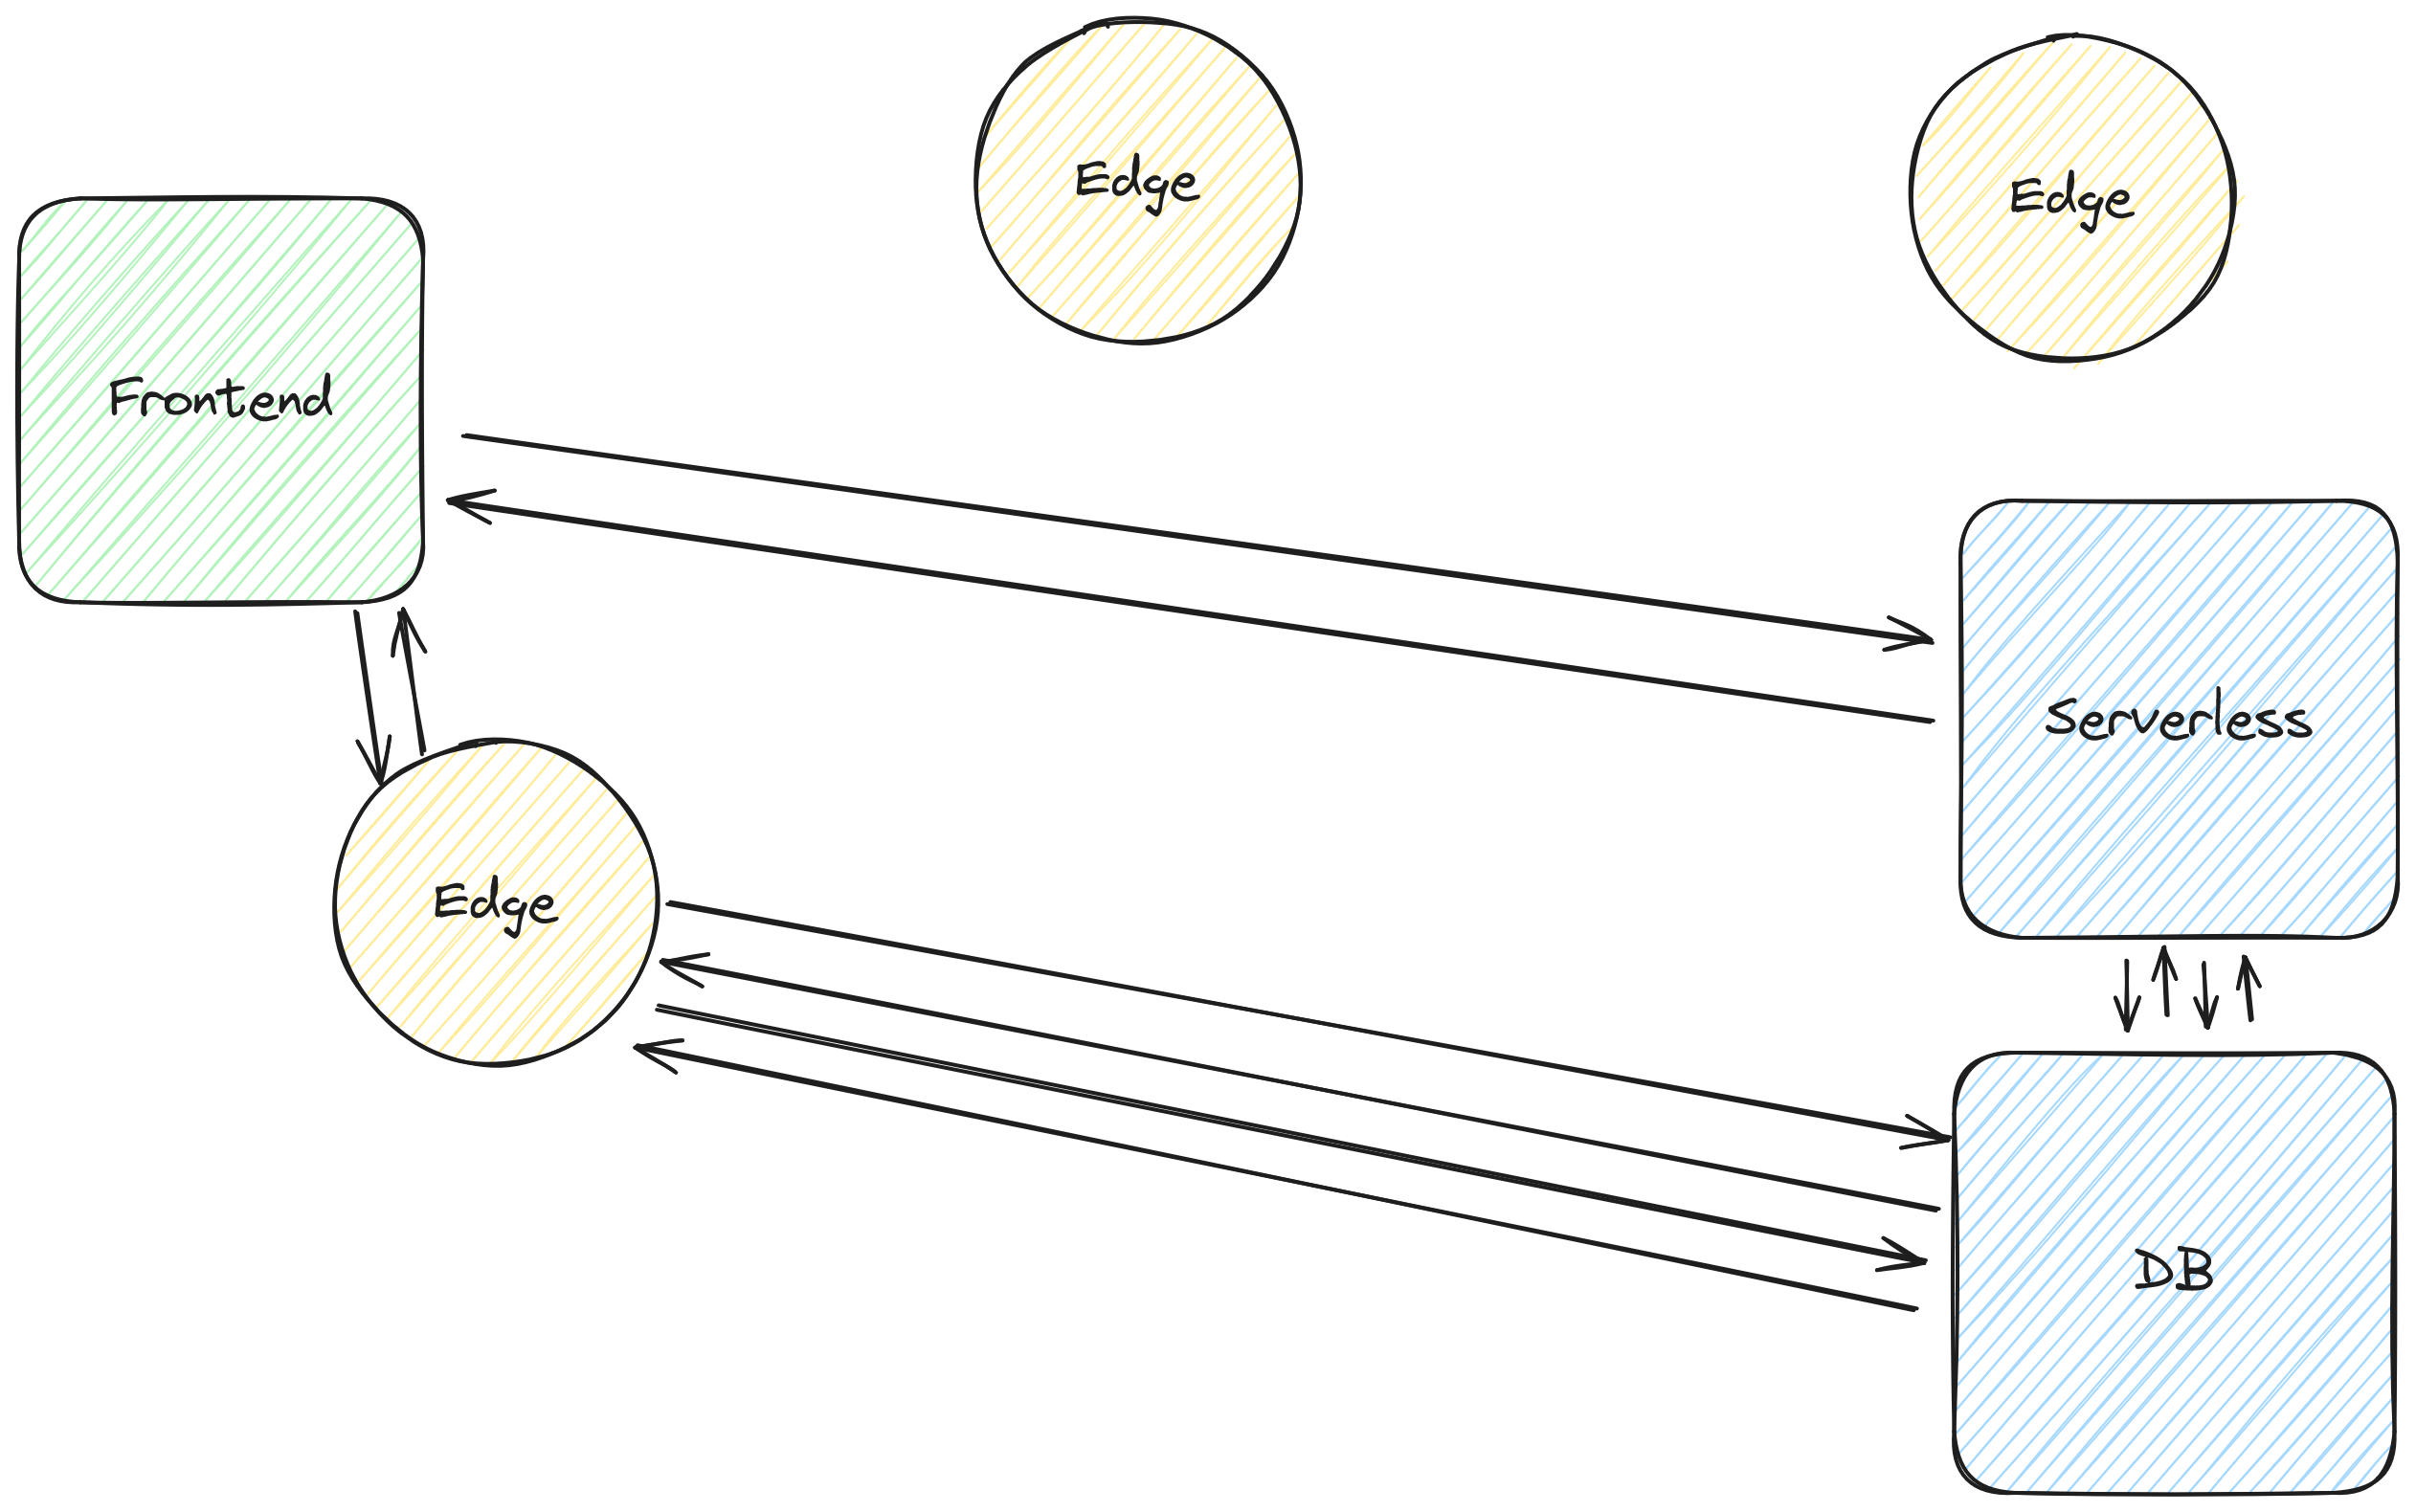
\includegraphics[width=0.7\linewidth]{image/edge-serverless.png} 
	\caption{Rozdíl mezi serverless a edge.} %% popisek obrázku, nezapomeň na citace!
	\label{fig:edge-serverless} %% označení až budeš chtít na obrázek odkazovat
\end{figure}

\item Metaframework je technologie, která kombinuje výhody \uv{single page application} a tradičního web serveru. Disponuje možností běhu kódu na serveru, přesměrováním na klientské části a dalšími výhodami. Takových technologií existuje celá řada, jako například populární NextJS, já si pro svůj projekt zvolil SvelteKit. Další fází této architektury je hostování, nejlepší variantou většinou bývá hostování přes providery jako Vercel nebo Netlify, tato architektura se poté spíše primárně aplikuje se \uv{serverless}.
\end{itemize}

Jednou z hlavních myšlenek bylo hostování Effia na cloudových službách, proto jsem si vybíral hlavně mezi technologiemi \uv{serverless} a \uv{edge computing}, výhodou providera, kterého jsem si vybral - Vercel je, že kombinace těchto technologií je velice snadná, základní variantou je \uv{serverless} s~jednoduchým přepnutím dané cesty na \uv{edge}. Ve spojení s~konceptem metaframeworku nakonec utváří velmi flexibilní, rychlou a příjemnou variantu.

%\begin{figure}[h!]
%	\centering %% příkaz, který ti obrázek zarovná na střed
%	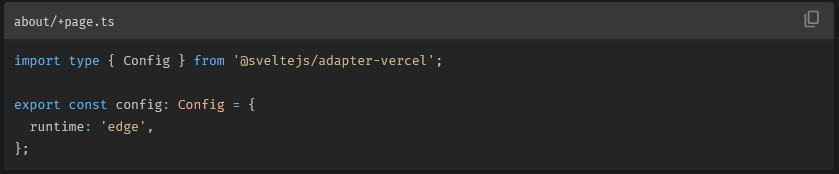
\includegraphics[width=1\linewidth]{image/edge-adapter.png} 
%	\caption{Možnost přepnutí dané cesty ze Serverless na Edge. \cite{SvelteKit}} %% popisek obrázku, nezapomeň na citace!
%	\label{fig:edge-adapter} %% označení až budeš chtít na obrázek odkazovat
%\end{figure}

%Vzhledem k tomu, že záměrem bylo vytvořit aplikaci, která bude pro veškeré \uv{backendové} úlohy využívat cloud, tak je architektura relativně složité téma, proto se pokusím stručně popsat základní proces vykreslení stránky. Uživatel získává statické soubory ze \uv{CDN}, dynamicky vytvořené stránky pro první zobrazení (\uv{first render}) jsou generovány na instancích \uv{serverless funkcí} třetí strany, každá instance se vytváří podle potřeby na reálném serveru poskytovatele, není dedikovaná a ani nezůstavá aktivní po delší dobu. Server je dále využíván pro potřeby klienta, které si on sám nemůže obstarat především z bezpečnostních důvodů (DB queries, secret env variables...). Databáze vytváří spojení se serverem a ten získává potřebná data.

\section{Typesafety}
\label{sec:typesafety}

Webové aplikace standardně využívají JavaScript, který ale přináší signifikantní nevýhodu v~podobě nemožnosti \uv{otypovat} kód. To způsobuje obtížnou orientaci v~kódu, vysoké množství produkčních chyb a také mnoho času stráveného pochopením dříve napsaného kódu. Pro Effio jsem se tedy rozhodl využít moderní technologie a vytvořit téměř plně \uv{typesafe} (otypovanou) aplikaci. TypeScript v~Effiu nahrazuje JavaScript a do tohoto jazyka přináší typovou strukturu. To však nestačí, protože API endpointy a databázové dotazy stále nemohou být otypované. Proto jsem přidal také knihovny tRPC a Prisma.

\section{Datové modely}
\subsection{Model Moodlu}
Pro import a export testů v rámci platformy Moodl, je využíván formát GIFT, ten obsahuje speciální syntaxi v~rámci textového souboru pro záznam jednotlivých otázek, k~zajištění konverze tohoto formátu do JSON, se kterým se dá dobře pracovat jsem využil knihovnu \texttt{gift-pegjs}, pokud ale šlo o konverzi opačnou, tedy z~JSON do GIFTu, rozhodl jsem se o napsání vlastní malé knihovny pro generaci daného souboru \texttt{gift-format-generator}.

\subsection{Datový model testu v Effiu}
Pro práci s~testem v~rámci Effia jsem se ale rozhodl pro vytvoření vlastního formátu, ve kterém by byl test uchováván ve \uv{storu} (objektu) až do jeho uložení do databáze.

\begin{lstlisting}[style=ES6, caption=Ukázka z +page.server.ts, label=test_format]
	type ClientTest = {
		title: string;
		description: string;
		questions: QuestionClient[]; // Otázky mají poté dalších spoustu atributů
		errors: {
			title?: string;
			description?: string;
			markSystem?: {
				[Key in keyof MarkSystemJSON as Key extends "marks" ? never : Key]?: string;} & {	marks: {[Key in keyof MarkSystemJSON["marks"][number]]?: string;}[]
				};
			tagIds?: string[];
		};
	}
\end{lstlisting}

\section{Backend}

\subsection{Založení a konfigurace projektu}
Prvním krokem bylo založení projektu a stažení potřebných knihoven, které jsem plánoval využít. Kombinace mnou vybraných technologií nebyla kompletně konvenční, a proto jsem se v~některých případech musel obrátit na komunitou vytvořené adaptéry. Příkladem je například knihovna \texttt{trpc-sveltekit}, která propojuje SvelteKit a tRPC. Toto propojení je vytvořeno s ohledem na skutečnost, že tRPC je primárně navrženo buď jako samostatný server nebo jako implementace do Next.js.

\subsection{Architektura backendu}
\begin{figure}[h!]
	\centering %% příkaz, který ti obrázek zarovná na střed
	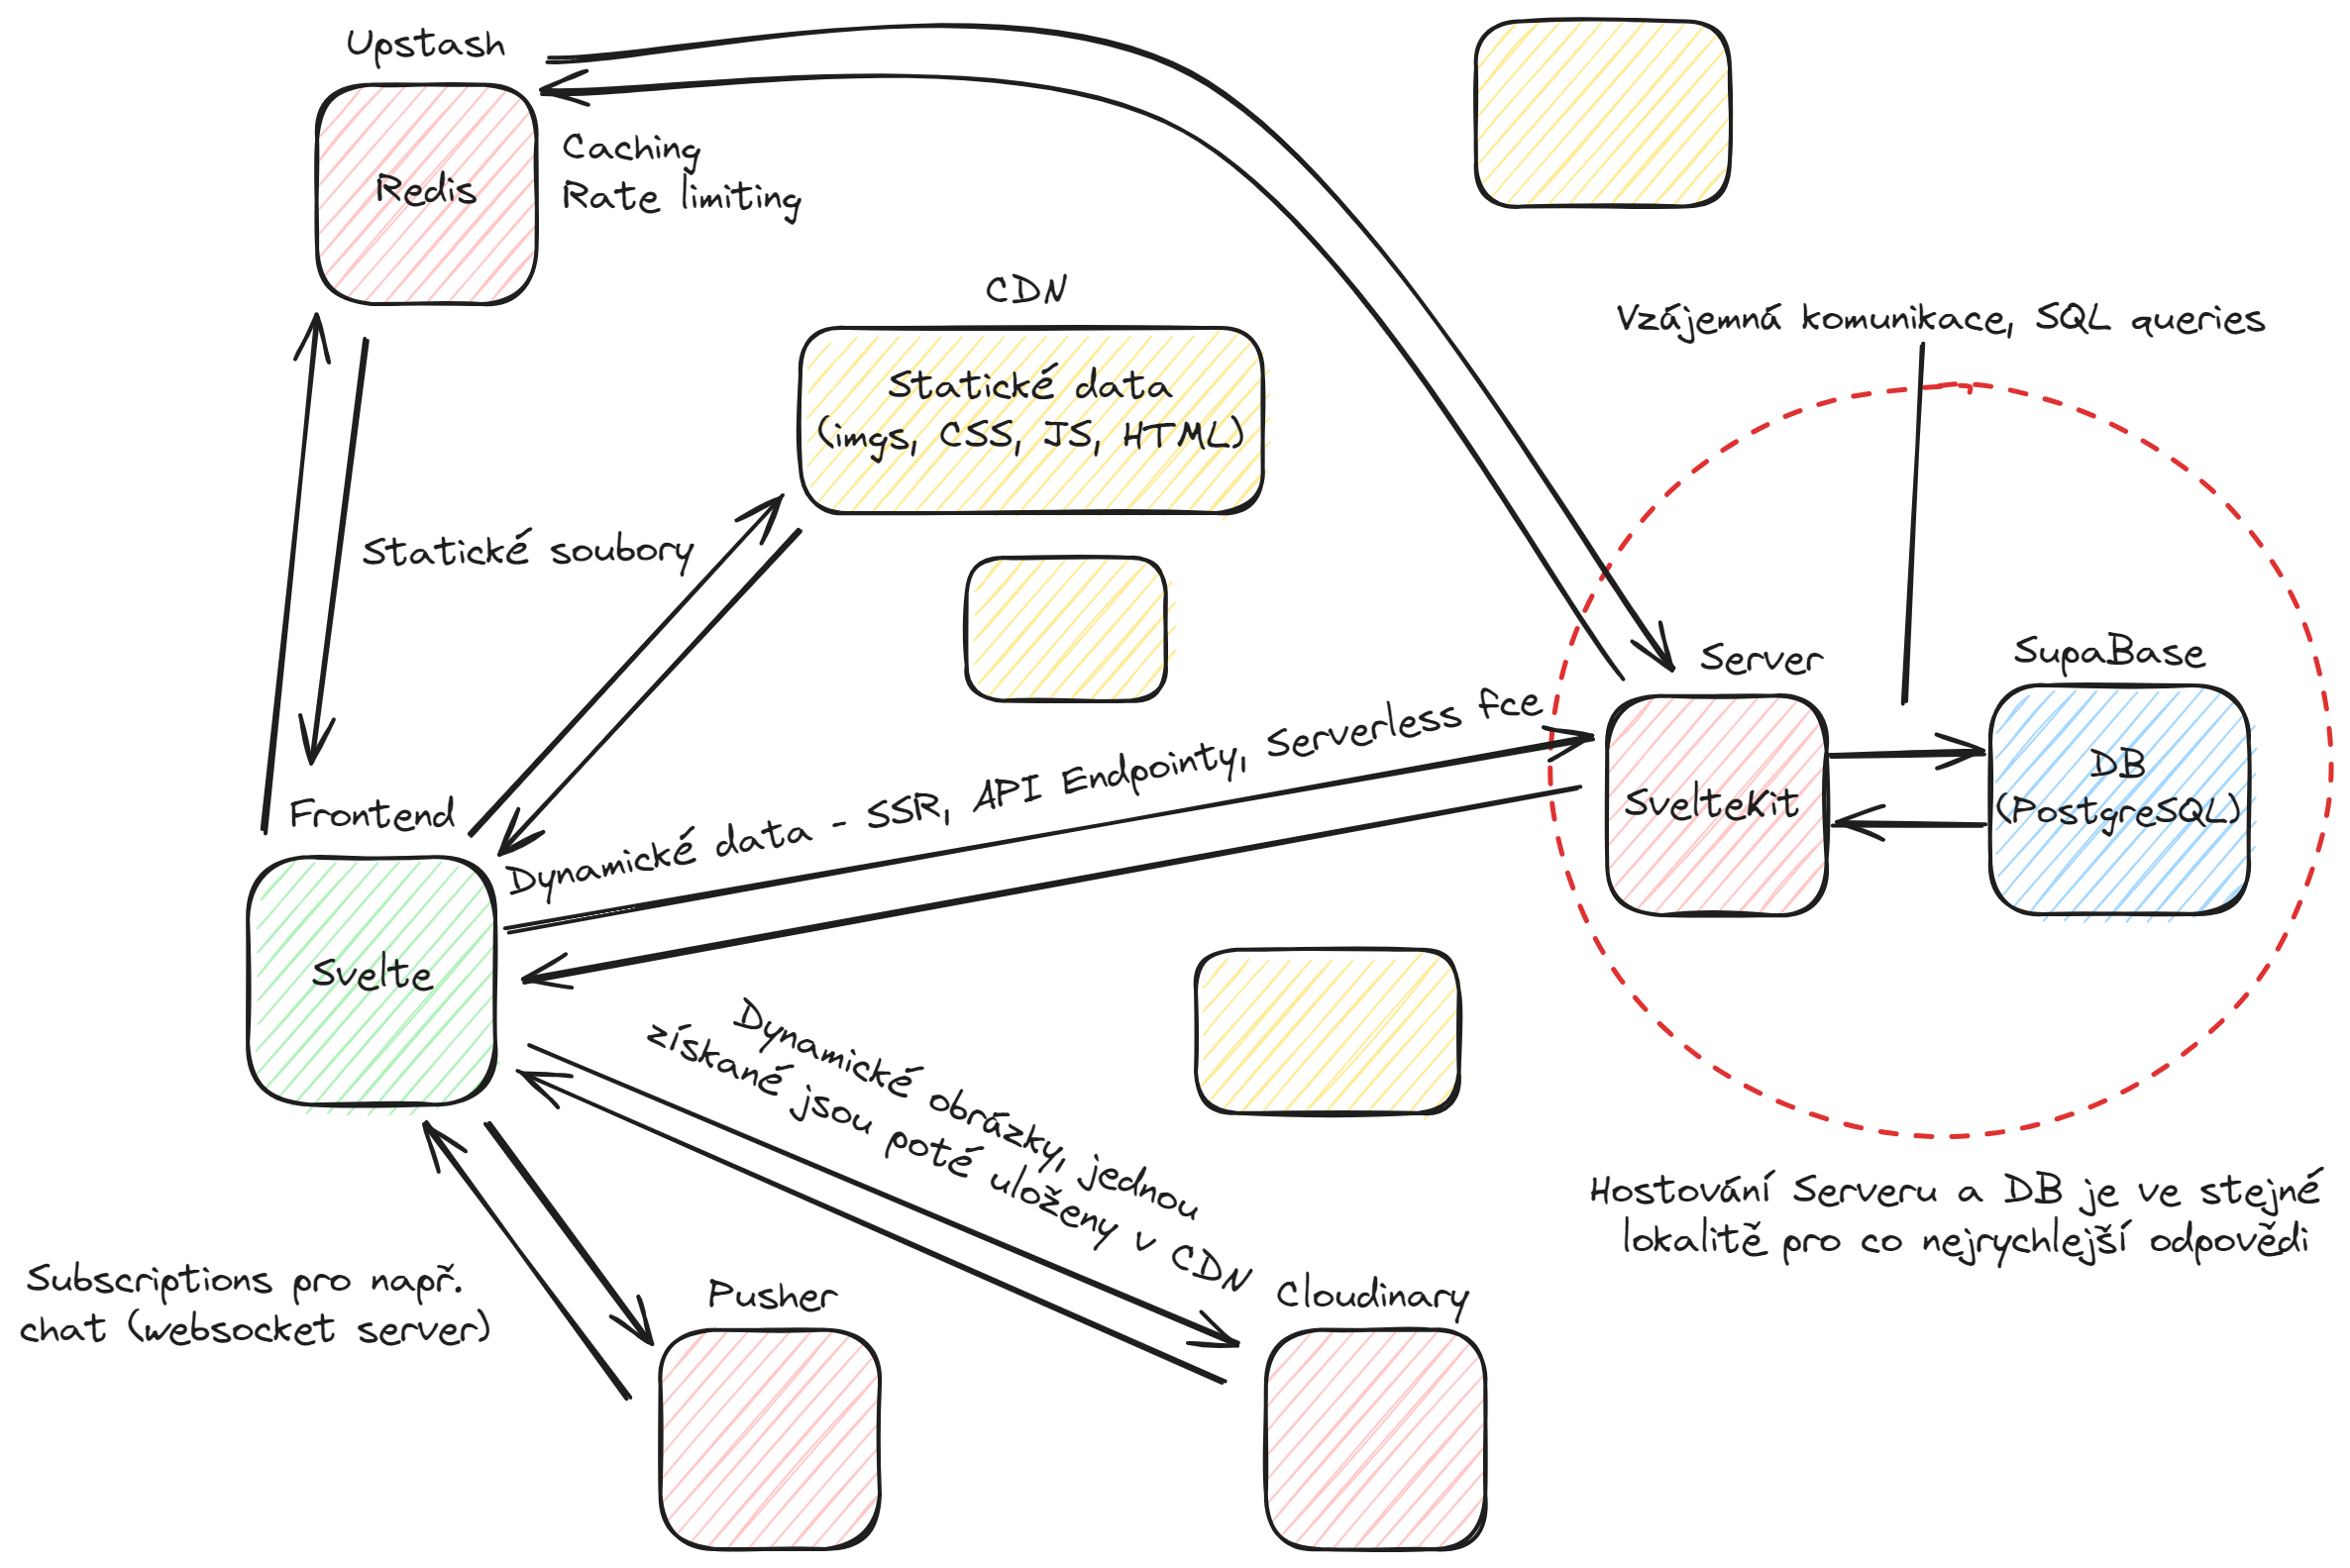
\includegraphics[width=1\linewidth]{image/effio-architecture.png} 
	\caption{Jednoduchý přehled backendové části Effia.} %% popisek obrázku, nezapomeň na citace!
	\label{fig:effio-architecture} %% označení až budeš chtít na obrázek odkazovat
\end{figure}

	\begin{itemize}
		\item CDN, neboli Content Delivery Network, je síť serverů, která je charakterizována zejména tím, že je rozmístěna po celém světě a ve velkém množství. Tato síť se stará o distribuci statického obsahu, čímž umožňuje klientům získávat data ze serverů, které jsou většinou mnohem blíže. Dále se CDN stará o cachování dat, což opět zkracuje dobu, po kterou uživatelé zobrazují obsah.
		\item Termín \uv{Server} neoznačuje server jako takový ale spíše místo kde se spouštějí instance serverových funkcí, což jsou funkce, které se vytváří podle potřeby na reálných serverech, které ale spravuje provider této služby, v~mém případě Vercel, respektive Cloudflare.
		
		Programátora nemusí tyto servery vůbec zajímat, instance se sami spouštějí, škálují a obecně jsou pro vývojáře velice příjemným řešením.
		
		Tento server je v~Effiu využíván hlavně pro první zobrazení stránky metodou SSR (\uv{server side rendering}) a také pro získávání dat, které nemohou být získány na klientu (např. SQL dotazy), pro jednotlivé stránky, formulářové akce nebo API endpointy.
		
		\item DB - PostgreSQL databáze hostovaná přes službu Supabase, ta nabízí mnoho nástrojů pro vývoj webových aplikací včetně databáze, je open source, má \uv{free tier} pro cloud hosting a nabízí také \uv{self hosting}.
		\item Pusher, Cloudinary, Upstash - jedná se o cloudové služby, které slouží účelům, které s~touto architekturou nejsem schopný zařídit.

		\begin{itemize}
			\item Pusher se stará o webové sockety, konkrétně o trvalé spojení, což není možné s~\uv{serverless} spojením. V~Effiu sloužil pro chat v~kanálech skupin pro aktualizaci zpráv všech uživatelů, když někdo odešle zprávu.
			
			\item Cloudinary slouží pro ukládání obrázků a jejich distribuci do CDN.
			
			\item Upstash je služba, která nabízí Redis instanci, kterou využívám pro caching a také \uv{rate limiting} (to znamená, že kontroluju počet requestů na jednotlivé endpointy). Redis je \uv{inmemory} databáze a hlavní výhodou je právě jeho rychlost.
		\end{itemize}
	\end{itemize}

\clearpage
\subsection{Autentifikace}
\subsection{Auth.js}

Auth.js je knihovna sloužící pro autentifikaci, poskytuje možnost \uv{session based}, to je použito v~Effiu, a JWT autentifikace. Dále knihovna podporuje OAuth s mnohými providery, v~tomto projektu je využit GitHub a Google s~jednoduchou možností přidat další. Výhodou knihovny je, že data si vývojář spravuje sám, neboli jsou ukládána do jeho vlastní databáze v~podobě tabulek (které si také může sám upravit): Account, Session, User a Verification Token, které poskytují naprostou kontrolu nad ověřením uživatelů.

\subsection{Proces přihlášení}
Uživatel, který se rozhodne přihlásit pomocí Google nebo GitHub účtu na podstránce /login, je následně přesměrován na stránky těchto providerů. Zde potvrdí přístup k~informacím o svém účtu a následně je vrácen zpět do Effia. V~databázi jsou vytvořeny tabulky o tomto uživateli, včetně nové relace (Session), díky které je schopen přihlášení. Tento proces probíhá automaticky po návratu uživatele zpět od providera.

\subsection{Databáze}

Jedná se o PostgreSQL databázi, která je hostovaná přes cloudovou platformu Supabase. Komunikace s~aplikací probíhá skrze ORM (Object-Relational Mapping), přesněji Prismu. Databázový model je umístěn jako příloha obrázku \ref{fig:schema}.

\subsection{Stručný popis účelů jednotlivých tabulek}

Autorizace a autentifikace
\begin{itemize}[itemsep=0pt]
	\item User - tabulka s údaji o uživateli.
	\item Account - účet uživatele, typ providera přes kterého je přihlášen a data k~relaci.
	\item Verification Token - ověřovací identifikátor providera.
	\item Session - relace, do jisté míry propojuje jednotlivé tabulky.
\end{itemize} 
Otázky
\begin{itemize}
	\item Question - otázka jako taková, obsahuje název, popis, její propojení s testy atd.
	\item QuestionType - typ otázky, rozhoduje jejím chování na frontendu.
	\item QuestionRecord - záznam otázky, po vyplnění testu se vytvoří ke každé otázce jeden nový záznam s~výsledky, je sdružován Test Recordem.
\end{itemize}
Testy
\begin{itemize}
	\item Test - obsahuje název testu, jeho popis a sdružuje veškeré další podrobnosti testu jako jsou Tagy, Stars, obsahuje množství TestVersion, což je vlastně jednotlivá verze testu.
	\item TestVersion - verze testu, uchovává odpovědi, body a Mark System, verze se aktualizují při každé změně testu.
	\item TestRecord - záznam vyplněného testu, obsahuje také Question Records.
\end{itemize}
Ostatní tabulky týkající se otázek
\begin{itemize}
	\item TestStar - ohodnocení testu hvězdičkou, každý uživatel mimo majitele může test takto ohodnotit, ekvivalent "liku" na sociálních sítích
	\item MarkSystem - známkovací systém daného testu, uživatel si ho může sám upravit a při uložení testu je uchovám právě v~této tabulce.
	\item Tag/TagOnTest - uchovává štítky týkající se tématu testu vybrané majitelem.
\end{itemize}
Skupiny
\begin{itemize}
	\item Group - skupina pro uživatele, obsahuje základní vlastnosti skupiny jako jméno, slug apod.
	\item GroupSubcategory - jednotlivý kanál skupiny, každý tento kanál má i samostatné zprávy, chat apod.
	\item GroupSubcategoryMessage - Zpráva v~kanálu, vztahuje se k~ní také její odesilatel, název, obsah atd. Obsahuje také MessageType, což je druh zprávy, kterou uživatel poslal.
\end{itemize}
Ostatní
\begin{itemize}
	\item Template - šablona testu
\end{itemize}

\subsection{Cloud hosting}
Jak již bylo zmíněno v~úvodu tak tato aplikace by se měla obejít bez vlastního serveru, nejde ale jenom o databázi ale také například o ukládání obrázků nebo hostování aplikace jako takové, to je prováděno přes \uv{Cloud hostingy} jako Vercel pro hostování stránky jako takové, zároveň ale řeší i rozesílání statických dat do CDN a poskytuje serverless lambda funkce, Supabase pro hostování mojí PostgreSQL databáze, Cloudinary, který slouží jako \uv{bucket} pro obrázky a také jejich možnost editace přes url parametry, Pusher který slouží jako web socket server například pro chat nebo Upstash, na kterém běží instance Redisu sloužícího pro caching a \uv{rate limiting}.

\subsection{Využité backendové technologie}

\subsubsection{SvelteKit}

SvelteKit je metaframework postavený nad Svelte, podobně jako ostatní metaframeworky slouží k~backendovým potřebám aplikace. Jeho hlavní výhody zahrnují:
\begin{itemize}
	\item Rychlost - Svelte vytváří velmi rychlé aplikace, a ve spojení s~Vitem (bundler) dosahuje také výborných výsledků v~rychlosti build procesu a \uv{hot module replacementu}. Rychlost vývoje je také podpořena minimálním množstvím \uv{boilerplate} kódu díky přístupu SvelteKitu.
	\item Flexibilita - SvelteKit umožňuje jednoduchou konfiguraci jednotlivých stránek nebo cest pro různé způsoby vykreslování, jako jsou SPA, SSR, SSG nebo MPA. Dále umožňuje variabilní kombinaci kódu běžícího na serveru a na klientovi, poskytuje rozsáhlou kontrolu nad jejich chováním a umožňuje snadné úpravy.
	\item Přehlednost - SvelteKit využívá \uv{file-based routing}, což znamená, že cesty aplikace jsou generovány podle složek vytvořených vývojářem. Soubory jsou následně pojmenovány konzistentně, například \texttt{+page.svelte} pro stránky a \texttt{+layout.svelte} pro layouty. Dalším prvkem přispívajícím k~přehlednosti je podobnost s~JavaScriptem, neboli to, že framework se snaží udržovat syntaxi velice podobnou čistému JavaScriptu.
\end{itemize} 

V~mé aplikaci SvelteKit zastává naprosto zásadní roli, od routování, přes serverové operace jako load funkce a API endpointy, konfiguraci bundleru až po přesměrování. Ve zkratce se jedná o základní stavební blok, bez kterého by aplikace nebyla funkční.

Tento kód ukazuje získání dat z~databáze při načtení stránky, ale před zobrazením uživateli, (load funkce) a poté také actions, což jsou formulářové akce vytvářené pro specifickou cestu, které poté můžeme využívat, zde je vidět mazání uživatele ze skupiny
\clearpage
\begin{lstlisting}[style=ES6, caption=Ukázka z +page.server.ts, label=sveltekit_code]
export const load: ServerLoad = async (event) => {
	// Mohou se vracet i Promisy, SvelteKit je sám resolvne, mění se ve SvelteKit 2.0
	const users = prisma.user.findMany({ where: {name: event.params.name}})
	return users
}
export const actions: Actions = {
	deleteUsers: async (event) => {
		const formData = await event.request.formData()
		const users: string[] = []
		formData.forEach((value) => { users.push(value.toString()) })
		try {
			await (await trpcServer(event)).groups.kickUsersFromGroup({
				groupSlug: event.params.name as string,
				userIds: users,
			})
			return { success: true }
		}
		catch (e) {
			if (e instanceof TRPCError) {
				return fail(getHTTPStatusCodeFromError(e), { message: e.message })
			}
			else { return fail(500, { message: "Something went wrong." }) }
		}
	}
}
\end{lstlisting}

\subsection{tRPC}
V~minulé kapitole jsem se zmínil o problémech s otypováním API endpointů, tRPC (Typescript Remote Procedure Call) tento problém řeší tím, že vytváří dynamické typy pro jednotlivé endpointy, podle toho jak si je sami nadefinujeme, ty se potom dají volat pomocí funkcí bez přímého použití \texttt{fetche} nebo třeba \texttt{axiosu} (tyto funkce ve skutnčnosti \uv{fetch} requesty vykonávají ale programátor se o ně nemusí starat přímo), tyto funkce jsou dokonale otypované a v~kódu tím pádem fungují jako jakákoliv jiná funkce vytvořená programátorem. Další výhodou je také to, že jednotlivé \uv{procedury}, což je vlastně API endpoint, mají k~dispozici metody pro kontrolu vstupu nebo třeba middleware, který například může zjišťovat stav přihlášení uživatele, jako zbytek knihovny jsou i tyto metody perfektně otypované.

V Effiu tRPC využívám hlavně jako možnost komunikace klienta s~databází, proces spočívá v~tom, že tRPC v~build timu vytvoří API endpointy, které poté klient přes zmíněné funkce volá. V~těchto endpointech se většinou nachází operace s~databází, ty na klientu provádět nemohu. Výhodou je, že tyto funkce mohu využívat i na serveru s~trochu odlišnou implementací.

Ukázka kódu zobrazuje vytvoření procedury, neboli endpointu, který se poté dá volat. V~druhé části je zobrazena právě zmíněná funkce, díky které získáme potřebné data.

\begin{lstlisting}[style=ES6, caption=Endpoint generovaný pomocí tRPC, label=trpc_code]
getTestById: procedure.input(z.object({
	id: z.string(),
	includeGroupSubcategories: z.boolean().optional()
})).query(async ({ ctx, input }) => {
	const test = await ctx.prisma.test.findUnique({
		where: { id: input.id },
		include: {
			subcategories: input.includeGroupSubcategories || false,
			owner: true,
			tags: {	include: { tag: true } },
			testVersions: {
				include: {
					questions: { include: { type: true } }
				},
				orderBy: { version: "desc" },
				take: 1
			}
		},
	})
	
	if (!test) return null
	return test
}),
\end{lstlisting}
\begin{lstlisting}[style=ES6, caption=Volání funkce pomocí tRPC klienta s metodou getTestById, label=trpc_code_use]
	const imageUrlToDeleteTest = await trpc($page).getTestById.query({
		id: props.data.id,
	})
\end{lstlisting}
\subsection{Prisma}
Prisma slouží jako ORM (Object–relational mapping), což umožňuje získávat data z~databáze pomocí JavaScriptu bez přímého použití jazyka SQL. Prisma se skládá z~klientské části, která komunikuje se serverovou částí pomocí protokolu založeného na JSON. Na serverové straně se následně vykonává SQL dotaz a odpověď je odeslána zpět klientovi. Prisma také řeší problémy s~otypováním dotazů. Je třeba definovat model databáze v~souboru \texttt{schema.prisma}, který popisuje její strukturu. Tento model může být používán jak pro generování dotazů, tak pro typování dat v~aplikaci.

Tato ukázka kódu zobrazuje SQL operaci, kterou Prisma vytvoří podle této objektové struktury, kterou jsem sestavil. Cílem je získat unikátní test pomocí jeho ID společně s~přidruženými tabulkami. Druhá ukázka poté vytváření modelu.

\begin{lstlisting}[style=ES6, caption=Získání testu podle id a přidání dat ze spojených tabulek, label=prisma_code_use]
	const test = await ctx.prisma.test.findUnique({
		where: {id: input.id},
		include: {
			subcategories: input.includeGroupSubcategories || false,
			owner: true,
			tags: {	include: {tag: true} },
			testVersions: {
				include: { questions: { include: { type: true } } },
				orderBy: { version: "desc" },
				take: 1
			}
		},
	})
\end{lstlisting}

\begin{lstlisting}[style=ES6, caption=Schéma modelu verze testu, label=prisma_code_schema]
model Question {
	id        String           @id @default(uuid())
	title     String
	createdAt DateTime         @default(now())
	updatedAt DateTime         @updatedAt
	typeId    String
	testId    String
	content   Json
	points    Int              @default(0)
	type      QuestionType     @relation(fields: [typeId], references: [id], onDelete: Cascade)
	test      TestVersion      @relation(fields: [testId], references: [versionId], onDelete: Cascade)
	records   QuestionRecord[]
	
	@@index([typeId])
	@@index([testId])
}
\end{lstlisting}

\subsection{Zod}
Zod je validační knihovna, podobná například Yup. To znamená, že jejím úkolem je kontrolovat mnou vložené vstupy. Knihovna vrací úspěšnost a také chyby, na které během kontroly narazí. Její výhodou je možnost využít validačních schémat Zodu jako typů. Samotná validace funguje i jako \uv{type guard}, což znamená, že kontroluje a nastavuje typy u vložených proměnných.

Zod je v~Effiu využíván jak na backendu, tak na frontendu. Jeho umístění v backendové části je pouze z~důvodu, že validační operace častěji probíhají na serveru. Díky Zodu jsem schopen přehledným a spolehlivým způsobem kontrolovat data testů, formulářů apod. Zásluhou hezky formátovaných vrácených chyb je poté mohu bezproblémově zobrazovat uživatelům.

Tento kód kontroluje zdali vložený input odpovídá struktuře \uv{answerSchema}, popřípadě nastaví error do proměné, která se poté zobrazí klientovi.

\begin{lstlisting}[style=ES6, caption=Validace vstupu pomocí validační knihovny Zod, label=zod]
const answerSchema = z.string().min(ANSWER_MIN, `Answer has to be at least ${ANSWER_MIN} character long.`).max(ANSWER_MAX, `Answer can be max ${ANSWER_MAX} characters long.`)
const result = answerSchema.safeParse(content.answers[item].answer)
if (result.success === false) {
	content.answers[item].error = result.error.errors[0].message
}
\end{lstlisting}

%\section{Cloud provideři}
%Effia plně spoléhá na cloudové řešení, díky nim je jednoduché zprovoznit plně funkční stránku bez jakékoliv starosti o fyzický hardware, stejně jako o škálování zdrojů podle potřeby.
%\begin{itemize}
	%\item \textbf{Vercel} se stará o hostování aplikace jako takové, distribuci statického obsahu na %CDN a jednoduše řeší znovuvytvoření stránky po změně kódu v~GitHub repozitáři. Vercel podporuje %\uvserverless\uv architekturu v~podobě tradiční lambda funkcí. Jedná se o instance dané funkce, %která se spouští na serveru, není dedikovaná ale spouští se a vypíná podle vytížení.
%	\item \textbf{Cloudinary} slouží
%\end{itemize}

\section{Frontend}

\subsection{Design}
Jednou z~hlavních myšlenek bylo vytvořit pohledem přívětivou aplikaci, proto se návrh designu stál klíčovou částí pro stylově propracovanější prvky stránky. Pro tvorbu designu, stejně jako vytváření a úpravu potřebných obrázků jsem využil aplikaci Figma.
\begin{figure}[H]
	\centering %% příkaz, který ti obrázek zarovná na střed
	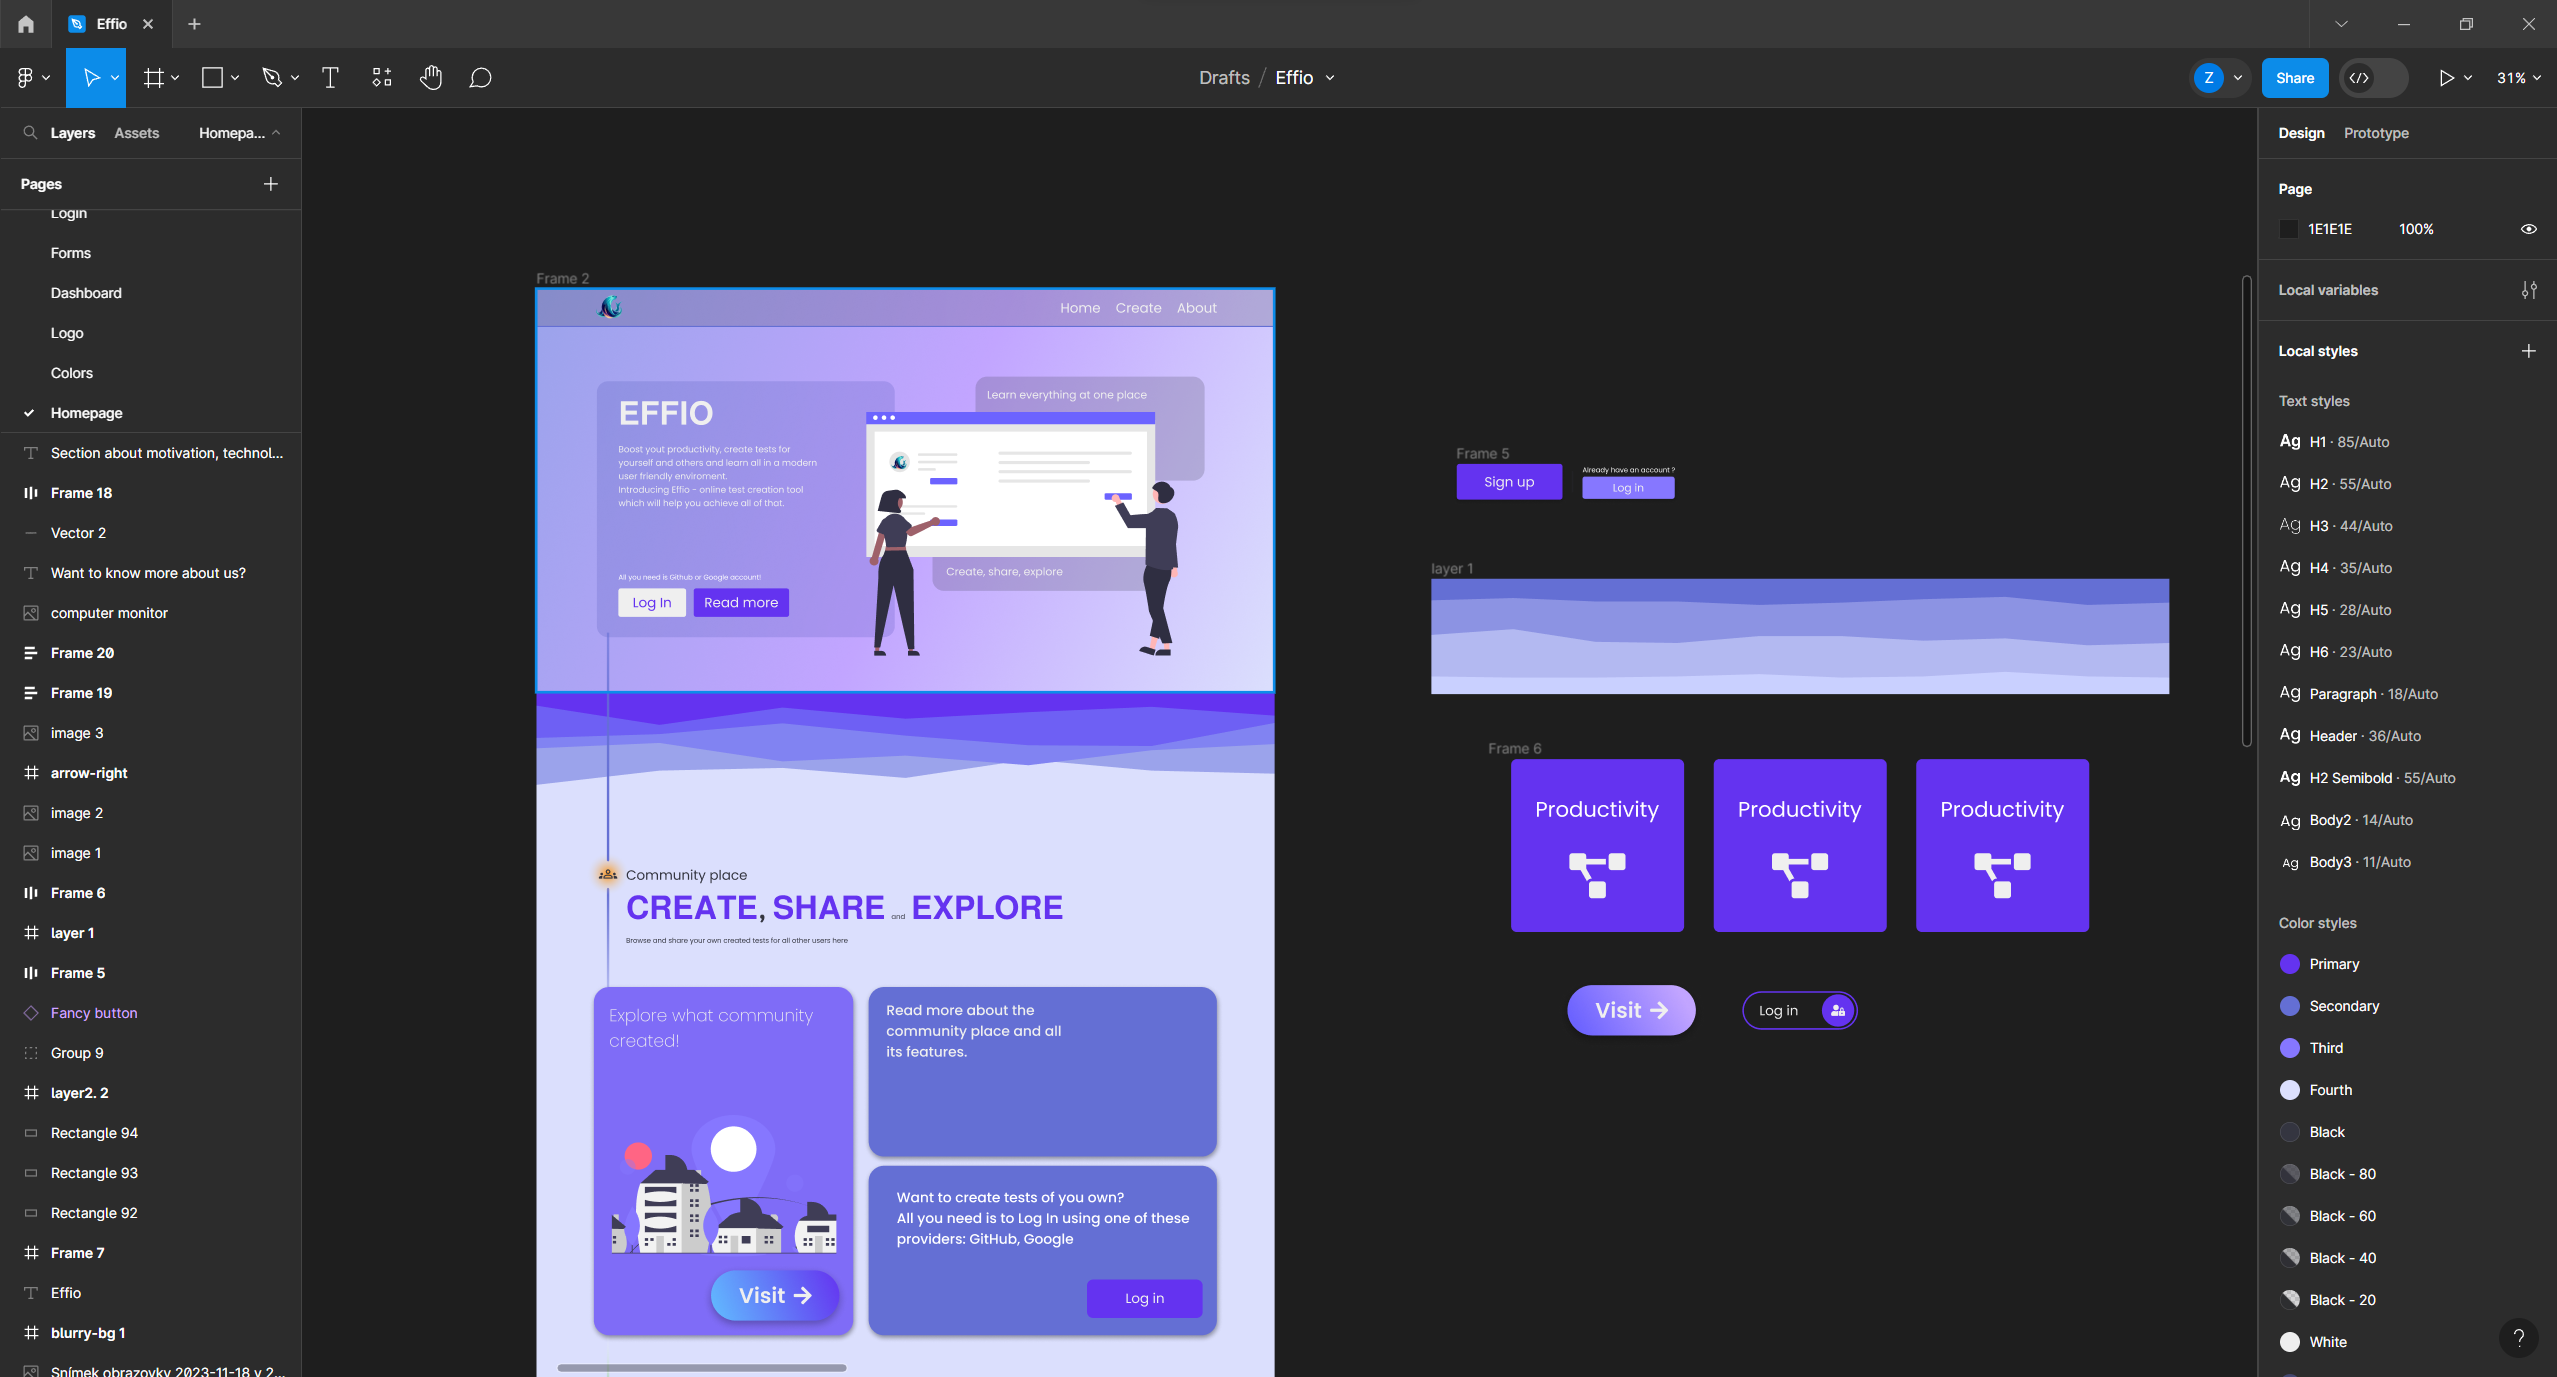
\includegraphics[width=0.8\linewidth]{image/figma.png} 
	\caption{Prvotní návrh domovské stránky.} %% popisek obrázku, nezapomeň na citace!
	\label{fig:figma} %% označení až budeš chtít na obrázek odkazovat
\end{figure}

\subsection{Responsivita}
Celá aplikace je uzpůsobená jak pro počítače tak pro mobilní zařízení. Responsivita není vůbec lehká práce, ale mně pomohl Tailwind. V něm se CSS media query dělají snadněji společně s moderními CSS kontejnery, které umožňují responsivní breakpointy odvozovat nejen od velikosti stránky, ale také od rozměrů rodičovských elementů.

Problematika však nespočívá pouze v~zobrazení prvků ale také v~jejich funkcionalitě, která musí fungovat jak s~myší, tak s~dotekem, příkladem tohoto problému je například jeden z~typů otázek, a to \uv{Connect}, kde se musí jednotlivé spoje přesouvat jak pohybem myši tak při dotykovém vstupu.

\begin{figure}[H]
	\centering
	\begin{minipage}[]{0.49\textwidth}
		\centering
		
\includegraphics[width=0.5\linewidth]{image/res1.png}
		\caption{Domovská stránka na mobilním zařízení}
		\label{fig:res1}
	\end{minipage}
	\hfill
	\begin{minipage}[]{0.49\textwidth}
		\centering
		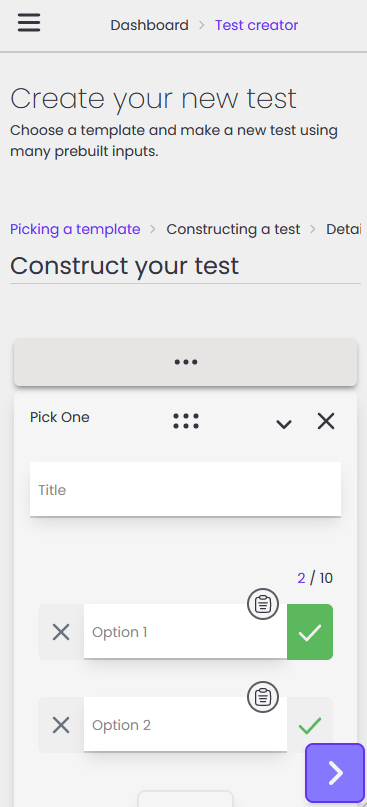
\includegraphics[width=0.5\linewidth]{image/res2.png}
		\caption{Generátor testů na mobilním zařízení}
		\label{fig:res2}
	\end{minipage}
\end{figure}

\subsection{Světlý a tmavý režim}
S~ohledem na uživatele, kteří preferují tmavý režim, jsem se také rozhodl vytvořit tmavý režim. Ten je možné vidět na obrázku \ref{fig:test-creator2}. Oba tyto režimy vyžadovaly vlastní paletu barev a byly mnohokrát přepracovány, aby jednotlivé barvy co nejlépe ladily k~sobě.

\subsection{Využité frontendové technologie}
\clearpage
\subsection{Svelte}
Svelte je open-source JavaScriptový framework vyvíjený týmem Riche Harrise od roku 2016. Jeho hlavní výhodou je rychlost a intuitivnost, protože jazyk, který používá, se snaží vypadat jako JavaScript, zatímco rozšiřuje jeho možnosti, tím se odlišuje od jiných framework jako je React, Angular, Solid nebo Qwik, ten se zapisuje do souborů s příponou .svelte. Tyto soubory jsou následně kompilovány do vysoce efektivního JavaScriptu. Díky tomu získává stále rostoucí popularitu mezi webovými vývojáři. Kód v~Svelte se skládá ze tří hlavních částí.

\begin{enumerate}
	\item Script - jedná se o část, kde se vypisují funkce, proměnné a řeší se reaktivní deklarace. Celá tato část je obklopená \texttt{<script>} tagy jako v~HTML dokumentu.
	\begin{lstlisting}[style=ES6, caption=Ukázka Svelte kódu ve script tagu, label=svelte-script-sample]
	export let inputValue: HTMLTextAreaElement['value'] = '';
	
	let setError = getContext('setError');
	
	let inputRef: HTMLTextAreaElement;
	
	const dispatch = createEventDispatcher();
	
	function validateInput() {
		const result = validationSchema?.safeParse(inputValue);
		if (!result?.success) {
			dispatch('error', result?.error.errors[0].message);
			if (typeof setError === 'function')
			setError(result?.error.errors[0].message);
		} else {
			dispatch('error', null);
			if (typeof setError === 'function') setError('');
		}
	}
	
	function dispatchInputChange() {
		dispatch('inputChange', inputRef.value);
	}
	\end{lstlisting}
	\item Style - tato část slouží jako CSS pro daný dokument. Výhodou je lokální rozsah aplikovaných stylů (podobný principu CSS modules), ale umožňuje i použití globálních stylů pomocí \texttt{:global}. Mě osobně vyhovuje, že se styly nacházejí v jednom souboru. I když jsem tento způsob pro stylování Effia převážně nevyužíval, osobně mi připadá velmi dobře provedený. Celý tento kódový úsek je formátován jako v HTML dokumentu a je obsažen v tagu \texttt{<style>}.
	
	\begin{lstlisting}[style=ES6, caption=Ukázka Svelte CSS kódu, label=svelte-CSS-sample]
	<style>
		.grid_cover {
			display: grid;
			grid-template-rows: auto 1fr;
		}
		:global(.dark) .fading {
			background-color: var(--dark-light_grey);
		}
	</style>
	\end{lstlisting}
	\item Obsahová část - vše, co se nenachází v jednom z~těchto tagů, představuje HTML reprezentaci dané stránky. Nejedná se však o čisté HTML, nýbrž obohacenou verzi. Podobně jako v~jiných frameworkách je možné přidávat \uv{event listenery} k~jednotlivým elementům, podmínkově je zobrazovat, pracovat s asynchronním kódem nebo dokonce \uv{svazovat} element nebo hodnotu elementu s~proměnnou ve scriptové části.
	
	\begin{lstlisting}[style=ES6, caption=Ukázka Svelte kódu, label=svelte-sample]
	{#await data}
		<!-- Zde se nachází další kód -->
	{:then awaitedData}
		<div class="@container h-full">
			<div
			bind:this={scrollerDiv}
			class="flex w-full h-full py-1 scroller flex-nowrap"
			style="--translate-x: 0%;"
			>
				{#each awaitedData as item}
					<div
					class="min-w-[calc(100%/var(--items-count))] relative aspect-[4/5]"
					>
						<CardAlternative
						navigationLink={'/tests/' + item.id}
						type={item.type}
						data={{...item}}
						/>
					</div>
				{/each}
			</div>
		</div>
	{/await}
	\end{lstlisting}
\end{enumerate}

\subsection{TypeScript}
Typescript lze považovat za nadstavbu JavaScriptu s~jednu výraznou výhodu - typy. Díky nim je mnohem snazší odhalovat chyby, vracet se k~dříve napsanému kódu a celkově zlepšit "developer experience" při vytváření aplikace. Sám o sobě dokáže pomoci s~otypováním jednotlivých částí kódu, ale nemá schopnost pracovat s~API endpointy nebo databázovými dotazy, které je nutné otypovat ručně. Z~tohoto důvodu jsou v~tomto projektu využívány další knihovny, jako jsou Prisma, tRPC a Zod.

V Effiu jsem se pro TypeScript rozhodl z~důvodů v sekci \ref{sec:typesafety}, zkráceně šlo ale hlavně o možnost efektivně psát kód, který bude obsahovat méně produkčních chyb, způsob jak se lépe vracet k~dřívějšímu kódu, také rychlost a jistota psaní, díky automatickému doplňování IDE, v~mém případě Visual Studio Codem.

Ukázka kódu zobrazuje vytváření různých typů, které poté v~aplikaci využívám.

\begin{lstlisting}[style=ES6, caption=Ukázka TypeScriptového typu, label=typescript-sample]
// Carousel.svelte
export type IdCardAlternativeProps = CardAlternativeProps & {
	id: string;
	type: TestType;
};

export type CarouselItemInput =
| IdCardAlternativeProps[]
| Promise<IdCardAlternativeProps[]>;

// customUtilities.d.ts

// Ručně vytvořený generic, který mi umožňuje zkombinovat funckionalitu Partial a Pick genericu. 
type PartialPick<T extends Record<unknown, unknown>, K extends keyof T> = {
	[Key in Exclude<keyof T, K>]: T[Key];
} & {
	[Key in K]?: T[Key];
}
\end{lstlisting}

\subsection{Tailwind CSS}
Tailwind CSS je utility knihovna pro práci s~CSS, která se odlišuje od frameworků jako Bootstrap nebo Material UI. Na rozdíl od nich neposkytuje celé předpřipravené komponenty, ale nabízí sadu připravených CSS tříd, které se aplikují na HTML elementy. Hlavní výhody Tailwind CSS spočívají v~absolutní kontrole nad chováním aplikovaných stylů, přehlednosti a rychlosti, s~jakou lze vytvářet styly.

Pro Effio jsem se rozhodl využít Tailwind především díky jeho flexibilitě a rychlosti použití. Pro některé komponenty jsem využil také Daisy UI, což je komponentová knihovna integrovaná s~Tailwind, pracující pouze s~CSS. Tato knihovna slouží jako plugin pro Tailwind.

Následující kód ukazuje, jak lze využít Tailwind tříd pro stylizaci určitého HTML elementu. I když jsem zde záměrně vybral rozsáhlejší příklad, většinou si vystačím s~jedním až dvěma řádky tříd.

\begin{lstlisting}[style=ES6, caption=Ukázka Tailwind kódu, label=tailwind-sample]
<button
	type="button"
	on:click={starTest}
	disabled={canStarTest === false || isSubmittingStar === true}
	class={`absolute flex items-center z-[2] gap-1 px-2 py-1 rounded-lg right-1 top-1 bg-light_white dark:bg-dark_grey shadow-md duration-100 ${
			isStarred ? 'bg-yellow-100 dark:bg-yellow-700' : ''
		} hover:bg-light_secondary dark:hover:bg-dark_secondary disabled:bg-light_grey_dark dark:disabled:bg-slate-600
		text-light_text_black dark:text-dark_text_white hover:text-light_whiter disabled:hover:text-light_text_black
		dark:disabled:hover:text-dark_text_white`}
	>
</button>
\end{lstlisting}

\chapter{Funkce aplikace}

%\section{Domovská stránka}
%Domovská stránka slouží jako prostor pro seznámení návštěvníka s~výhodami Effia. Nabízí rychlou navigaci mezi jednotlivými stránkami a je pečlivě navržena s~důrazem na design a efekty, aby zanechala dojem kvalitní aplikace.

%\begin{figure}[h]
%	\centering %% příkaz, který ti obrázek zarovná na střed
%	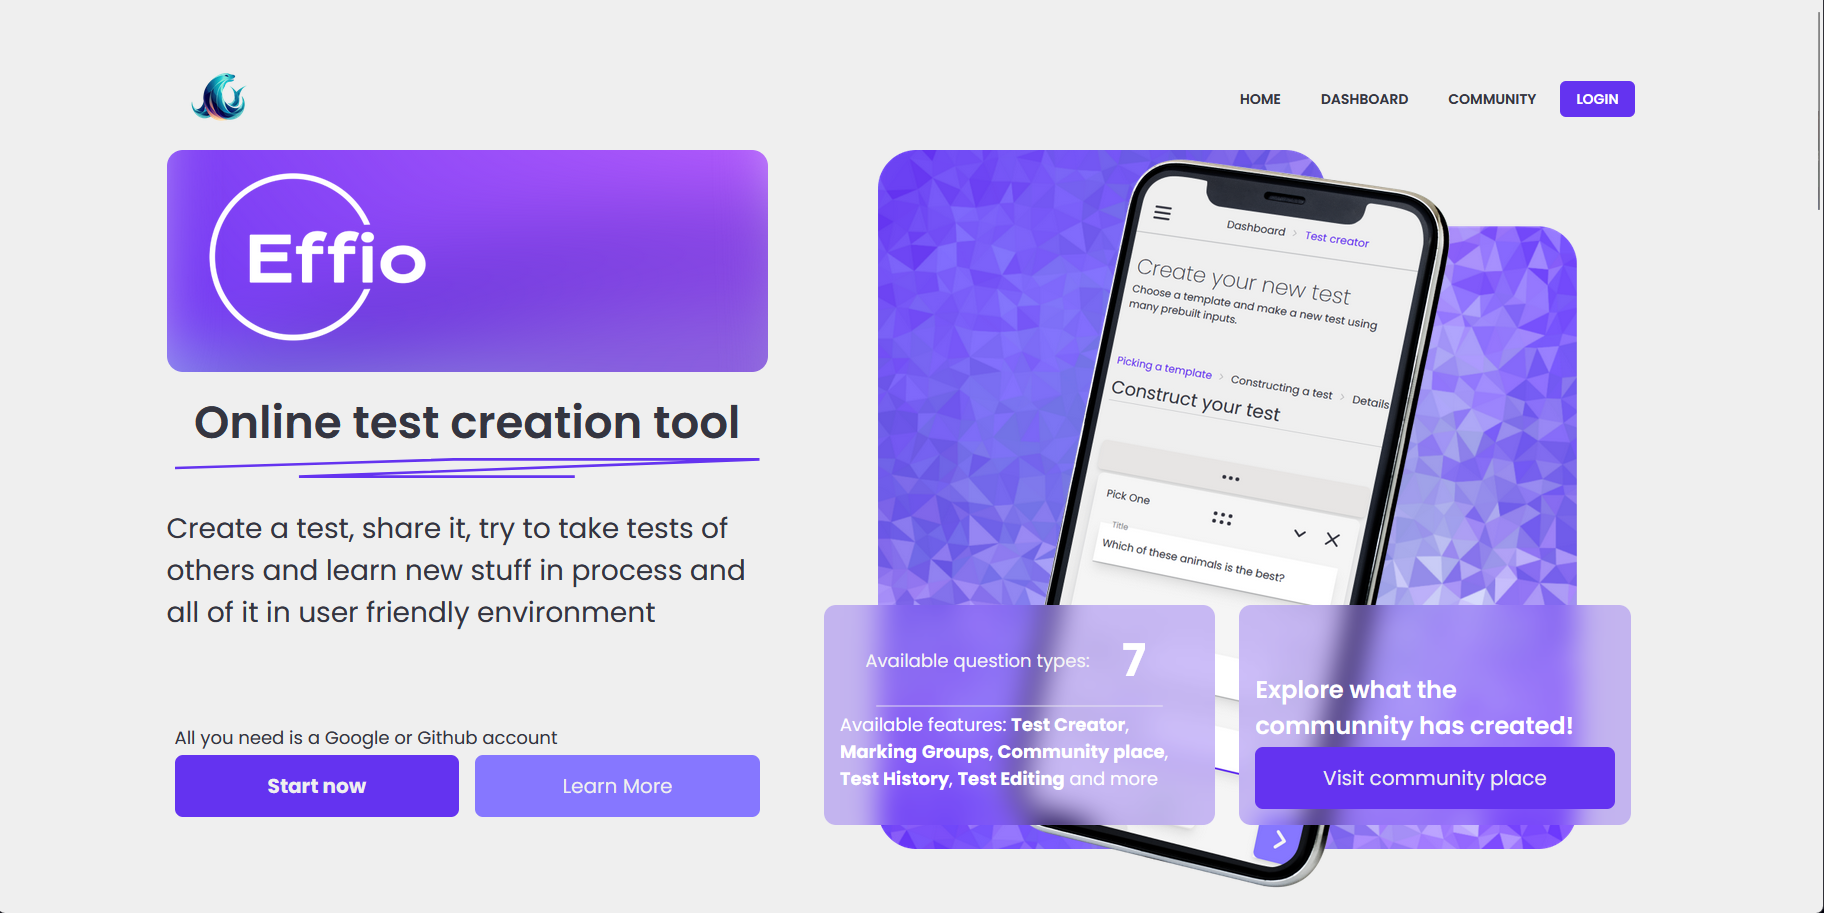
\includegraphics[width=1\linewidth]{image/homepage-notlogged.png} 
%	\caption{Domovská stránka Effia pro nepřihlášeného uživatele.} %% popisek obrázku, nezapomeň na citace!
%	\label{fig:homepage} %% označení až budeš chtít na obrázek odkazovat
%\end{figure}

\section{Přihlášení}
Po kliknutí na tlačítko \uv{Login} se dostanete na přihlašovací obrazovku, kde si můžete vybrat mezi přihlášením přes Google a GitHub účet. Po úspěšném přihlášení se uživatel dostane do dashboardu, který je spolu s~možností vytváření testů, prohlížením historie a správou skupin dostupný pouze pro přihlášené uživatele. Pokus o načtení stránky, pokud je uživatel nepřihlášený, vyústí v~přesměrování na přihlašovací stránku.

\begin{figure}[h]
	\centering %% příkaz, který ti obrázek zarovná na střed
	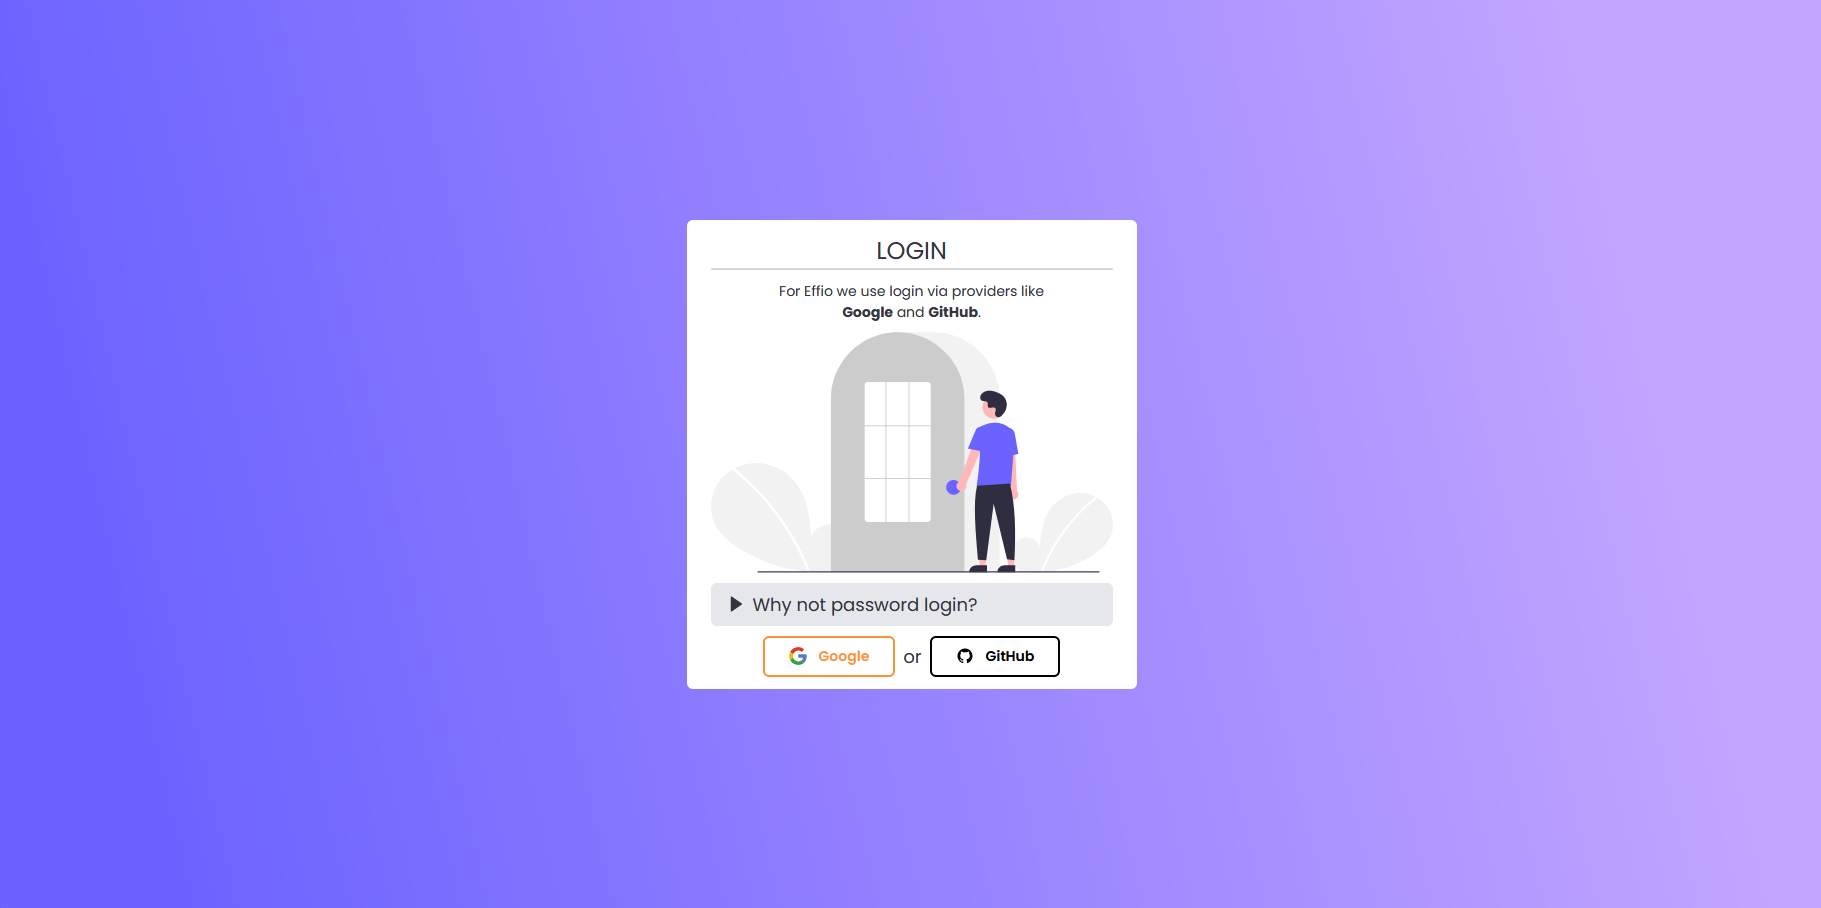
\includegraphics[width=1\linewidth]{image/login.png} 
	\caption{Domovská stránka Effia pro přihlášeného uživatele.} %% popisek obrázku, nezapomeň na citace!
	\label{fig:homepage-loggedin} %% označení až budeš chtít na obrázek odkazovat
\end{figure}

\subsection{Testy a jejich vlastnosti}
Jednou z esenciálních funkcionalit Effia je možnost vytvořit test. K~tomu existuje mnoho různých přístupů. Nejprve jsem se zamýšlel nad danou problematikou a až poté jsem napsal funkční nástroj pro jejich vytváření. Nicméně, i přes tuto předběžnou úvahu, bylo nakonec nutné téměř celou funkcionalitu při vytváření testu přepsat.

\subsubsection{Tvorba testu}
\label{subsec:creation}
Jako první si uživatel zvolí mezi kvízovým a programovacím testem, u obou si poté vybere šablonu.
\begin{itemize}
	\item Kvízový test: Po výběru šablony, která umožňuje i import z~formátu GIFT, se uživatel dostane do tvorby testu. Zde má možnost vybírat z~8~typů otázek: \textit{Pick One}, \textit{True/False}, \textit{Connect}, \textit{Write}, \textit{Fill}, \textit{Geography}, \textit{Image} a \textit{Bitmap}. Uživatel může libovolně měnit pořadí otázek, přidávat komentáře k~odpovědím a upravovat počet získaných bodů.
	\item Programovací test: Po výběru šablony se uživatel dostane do tvorby programovacího testu. Zde pojmenuje problém, popíše, co má uživatel řešit, nadefinuje kontrolní vstupy a očekávané výstupy. Dále může přidat nápovědy.
\end{itemize}
Po dokončení těchto úprav se uživatel přesune do konečných úprav testu, kde zadá jméno, popisek a přidá obrázek testu. Má možnost volitelně zařadit test do skupin, přidat tagy, rozhodnout se pro použití vlastního známkovacího systému (který si může upravit), zvolit náhodné třídění otázek a nakonec se rozhodnout, zda test uložit jako návrh nebo ho publikovat.

\begin{figure}[h]
	\centering
	\begin{minipage}[]{0.49\textwidth}
		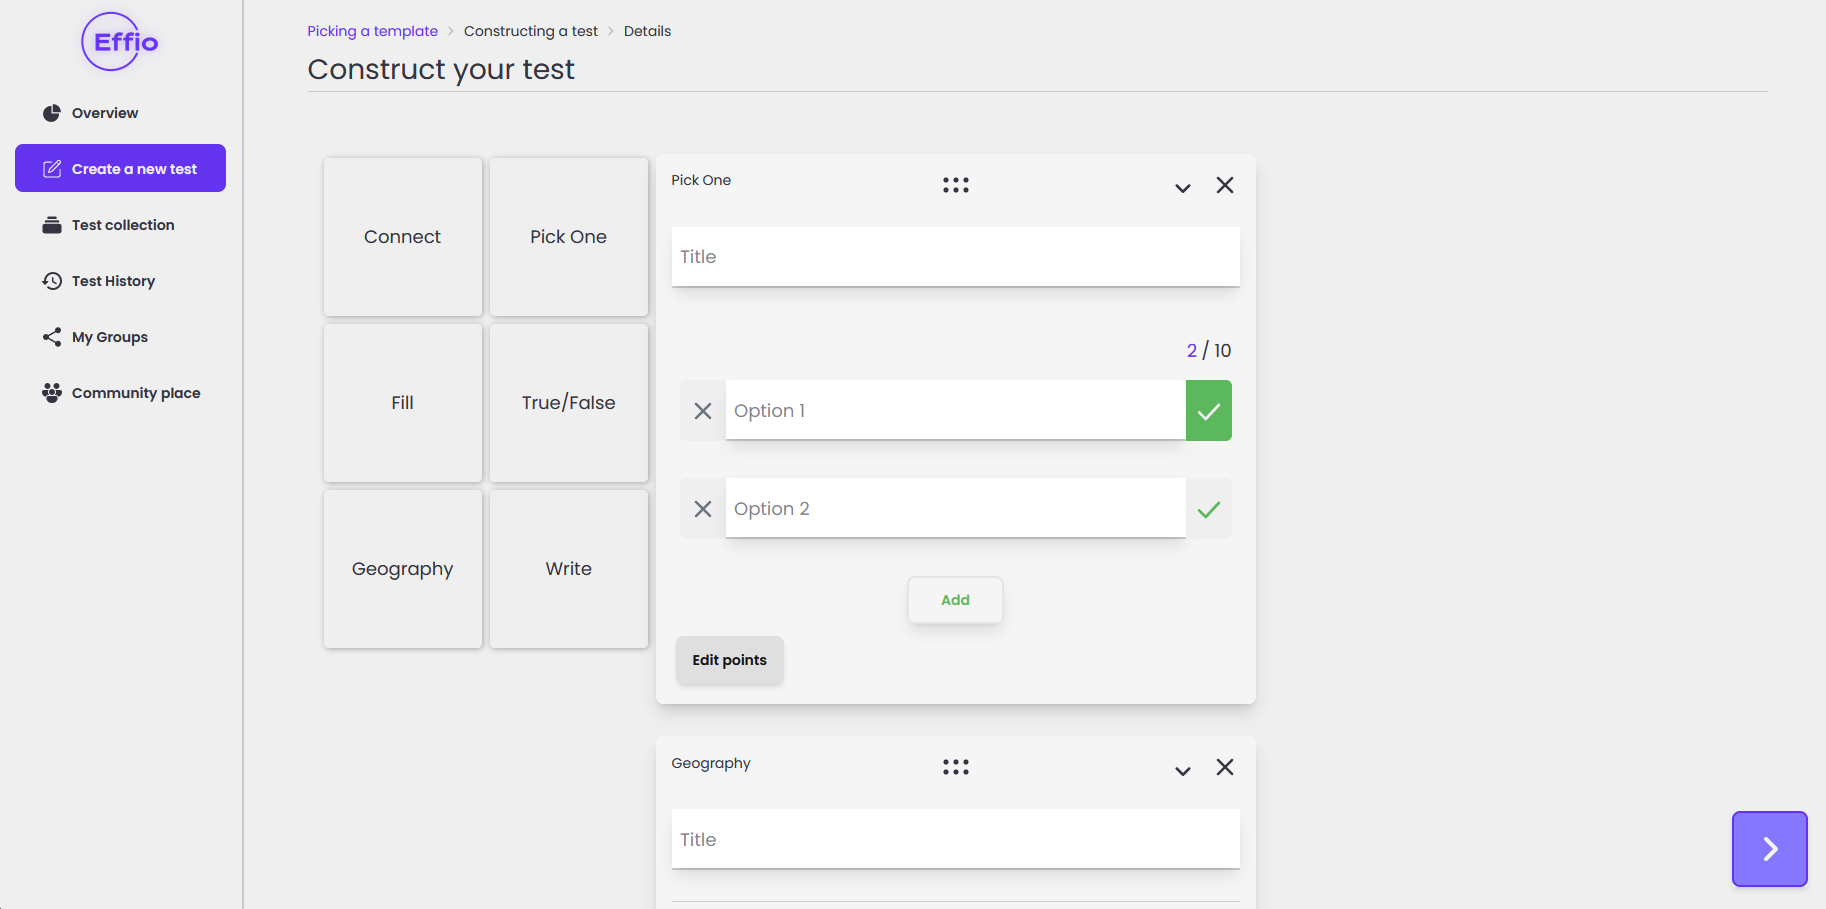
\includegraphics[width=\textwidth]{image/test-creator1.png}
		\caption{Kvízový test}
		\label{fig:test-creator1}
	\end{minipage}
	\hfill
	\begin{minipage}[]{0.49\textwidth}
		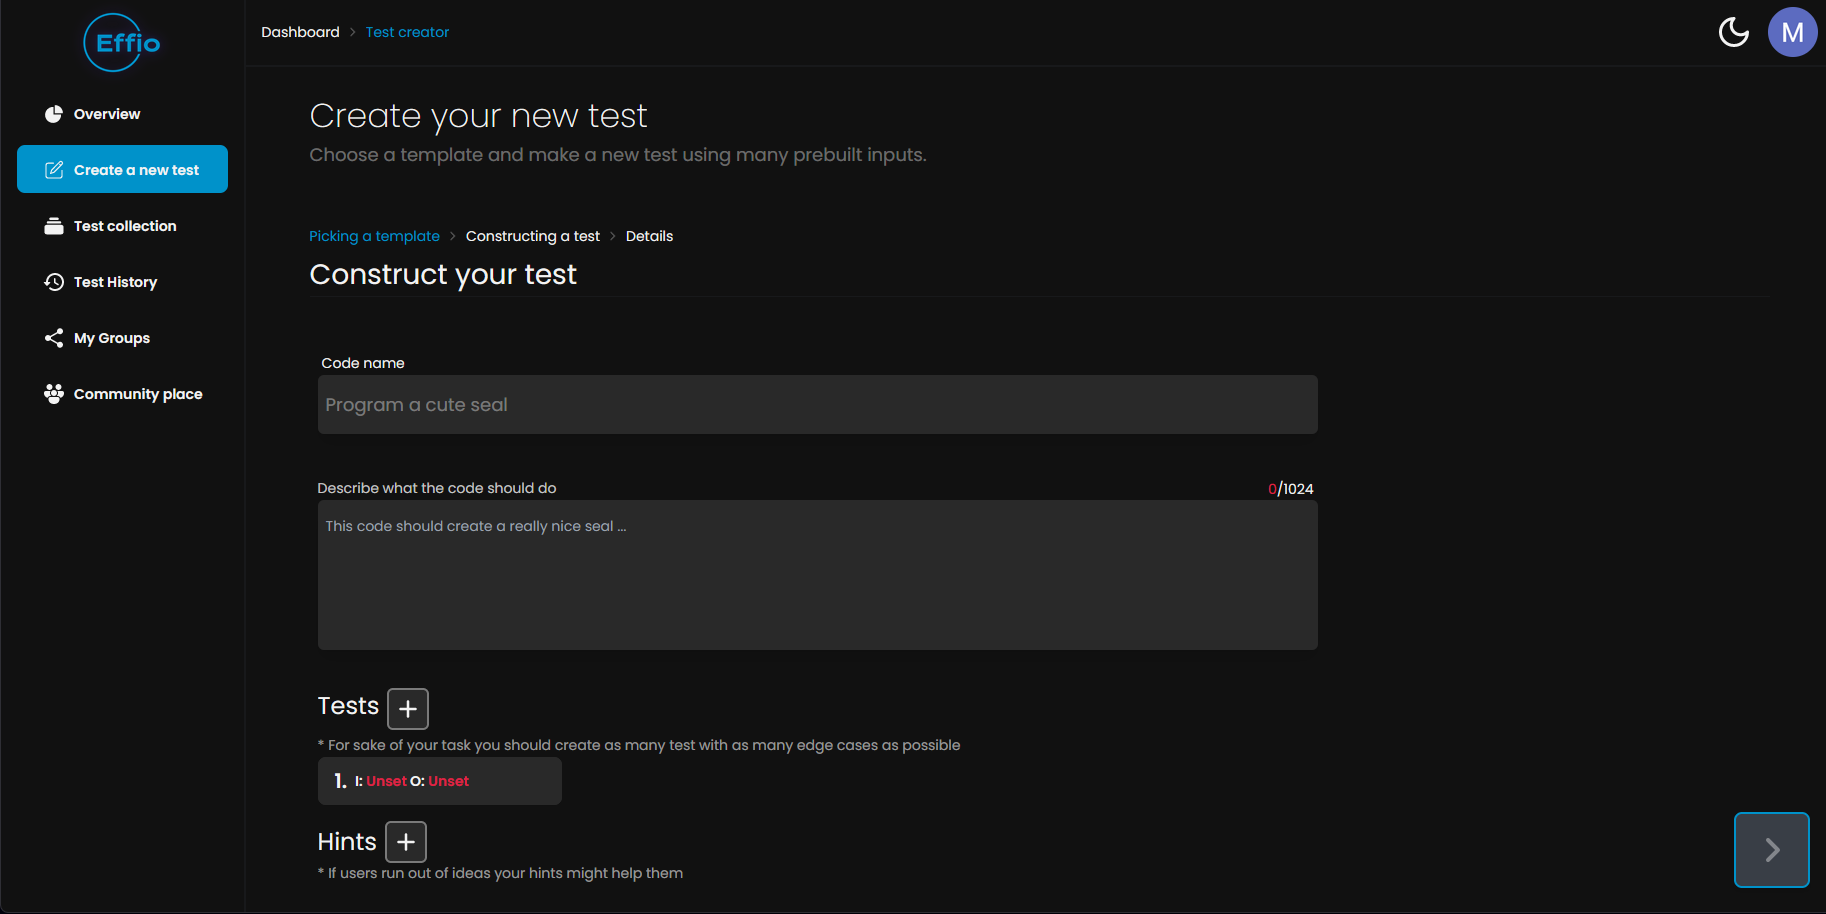
\includegraphics[width=\textwidth]{image/test-creator2.png}
		\caption{Programovací test}
		\label{fig:test-creator2}
	\end{minipage}
\end{figure}

\subsection{Vyplňování testu}
\label{sec:test-take}
\subsubsection{Vyplňování kvízu}
Vytvořený test si poté může kdokoliv s~přístupem k~němu vyplnit (testy jsou základně dostupné pro všechny, po úpravě mohou být zveřejněny pouze pro členy skupin).

Otázky jsou náhodně seřazeny, a uživatel musí odpovědět na všechny z~nich. Odpovědi některých typů otázek jsou náhodně zamíchány. Po vyplnění všech otázek uživatel odevzdá test, který se následně zkontroluje. Uživateli jsou zobrazeny správné odpovědi, počet získaných bodů, udělená známka a pokud je uživatel přihlášený, záznam o vyplnění se uloží do databáze. Uživatel si poté může zobrazit záznam v~sekci \textit{Test history}.

\begin{figure}[H]
	\centering %% příkaz, který ti obrázek zarovná na střed
	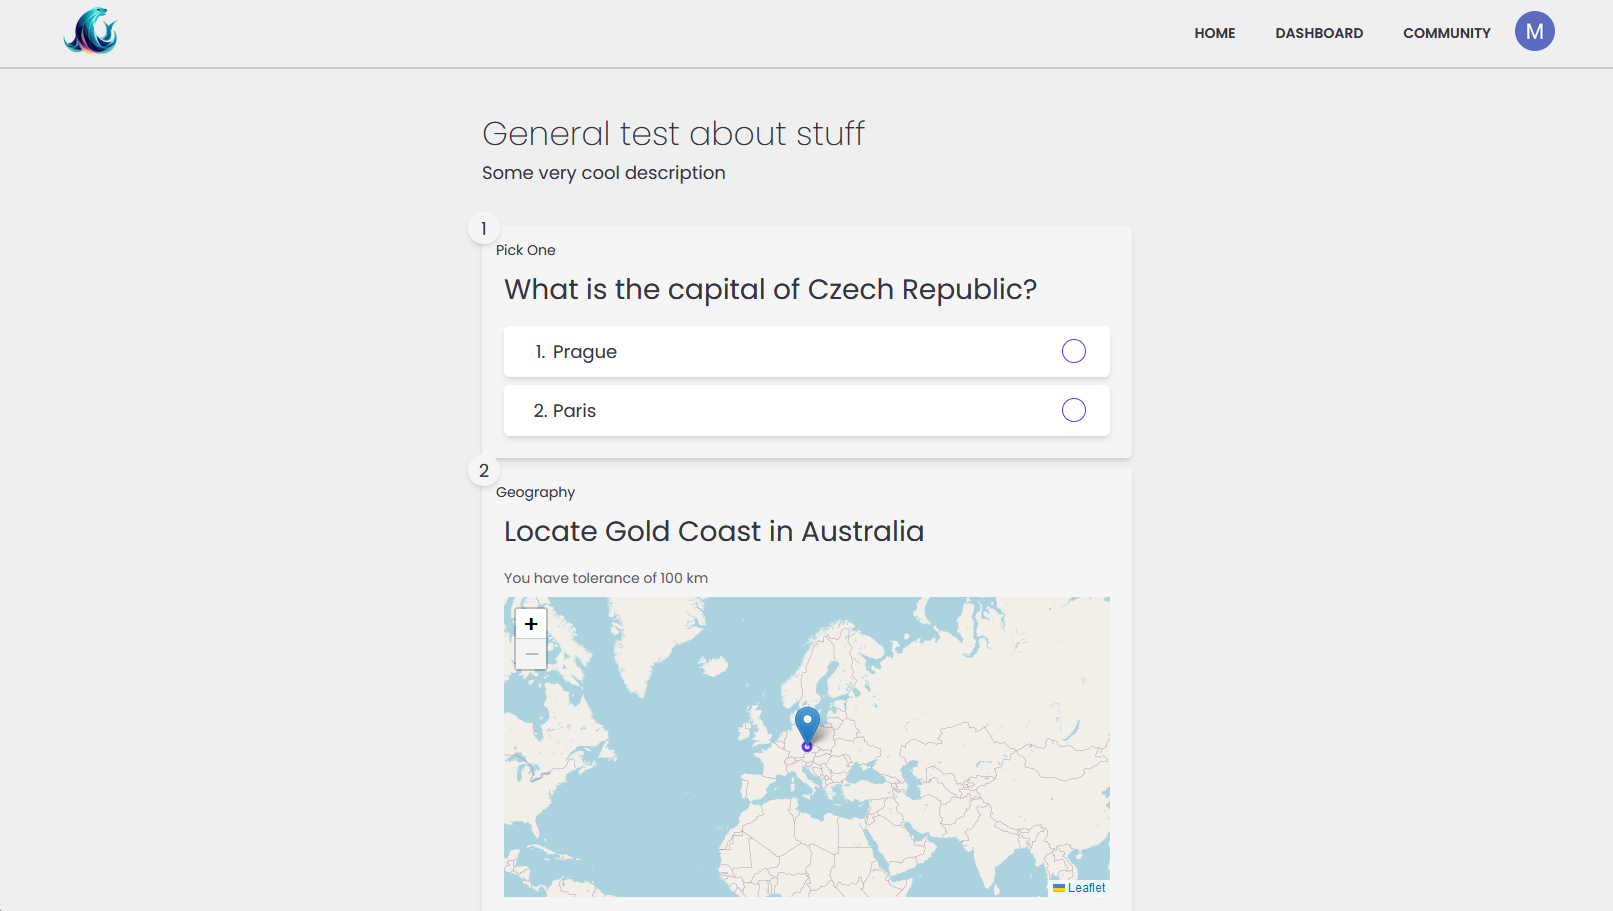
\includegraphics[width=0.75\linewidth]{image/test-taking.png} 
	\caption{Obrázek kvízu.} %% popisek obrázku, nezapomeň na citace!
	\label{fig:test-taking} %% označení až budeš chtít na obrázek odkazovat
\end{figure}

\subsubsection{Plnění programovacího testu}
Uživatel obdrží popis toho, co by měl kód schopný vykonat, sadu testů, které mají ověřit funkčnost kódu, a případné nápovědy. V~případě programovacích testů je k~dispozici vlastní editor, do kterého uživatel píše kód. Pro kontrolu správnosti kódu může použít tlačítko \textit{\uv{Run}} a v~případě, že testy procházejí, může odevzdat své řešení. Jednotlivý běh kódu probíhá na klientovi v~rámci \uv{web workerů}, které přesouvají zátěž na jiné vlákno procesoru, hlavní výhodou je ale, že pokud dojde k nějaké situaci, kterou nelze snadno vyřešit (třeba while true), tak je možné tento worker zrušit a spustit nový.

\begin{figure}[H]
	\centering %% příkaz, který ti obrázek zarovná na střed
	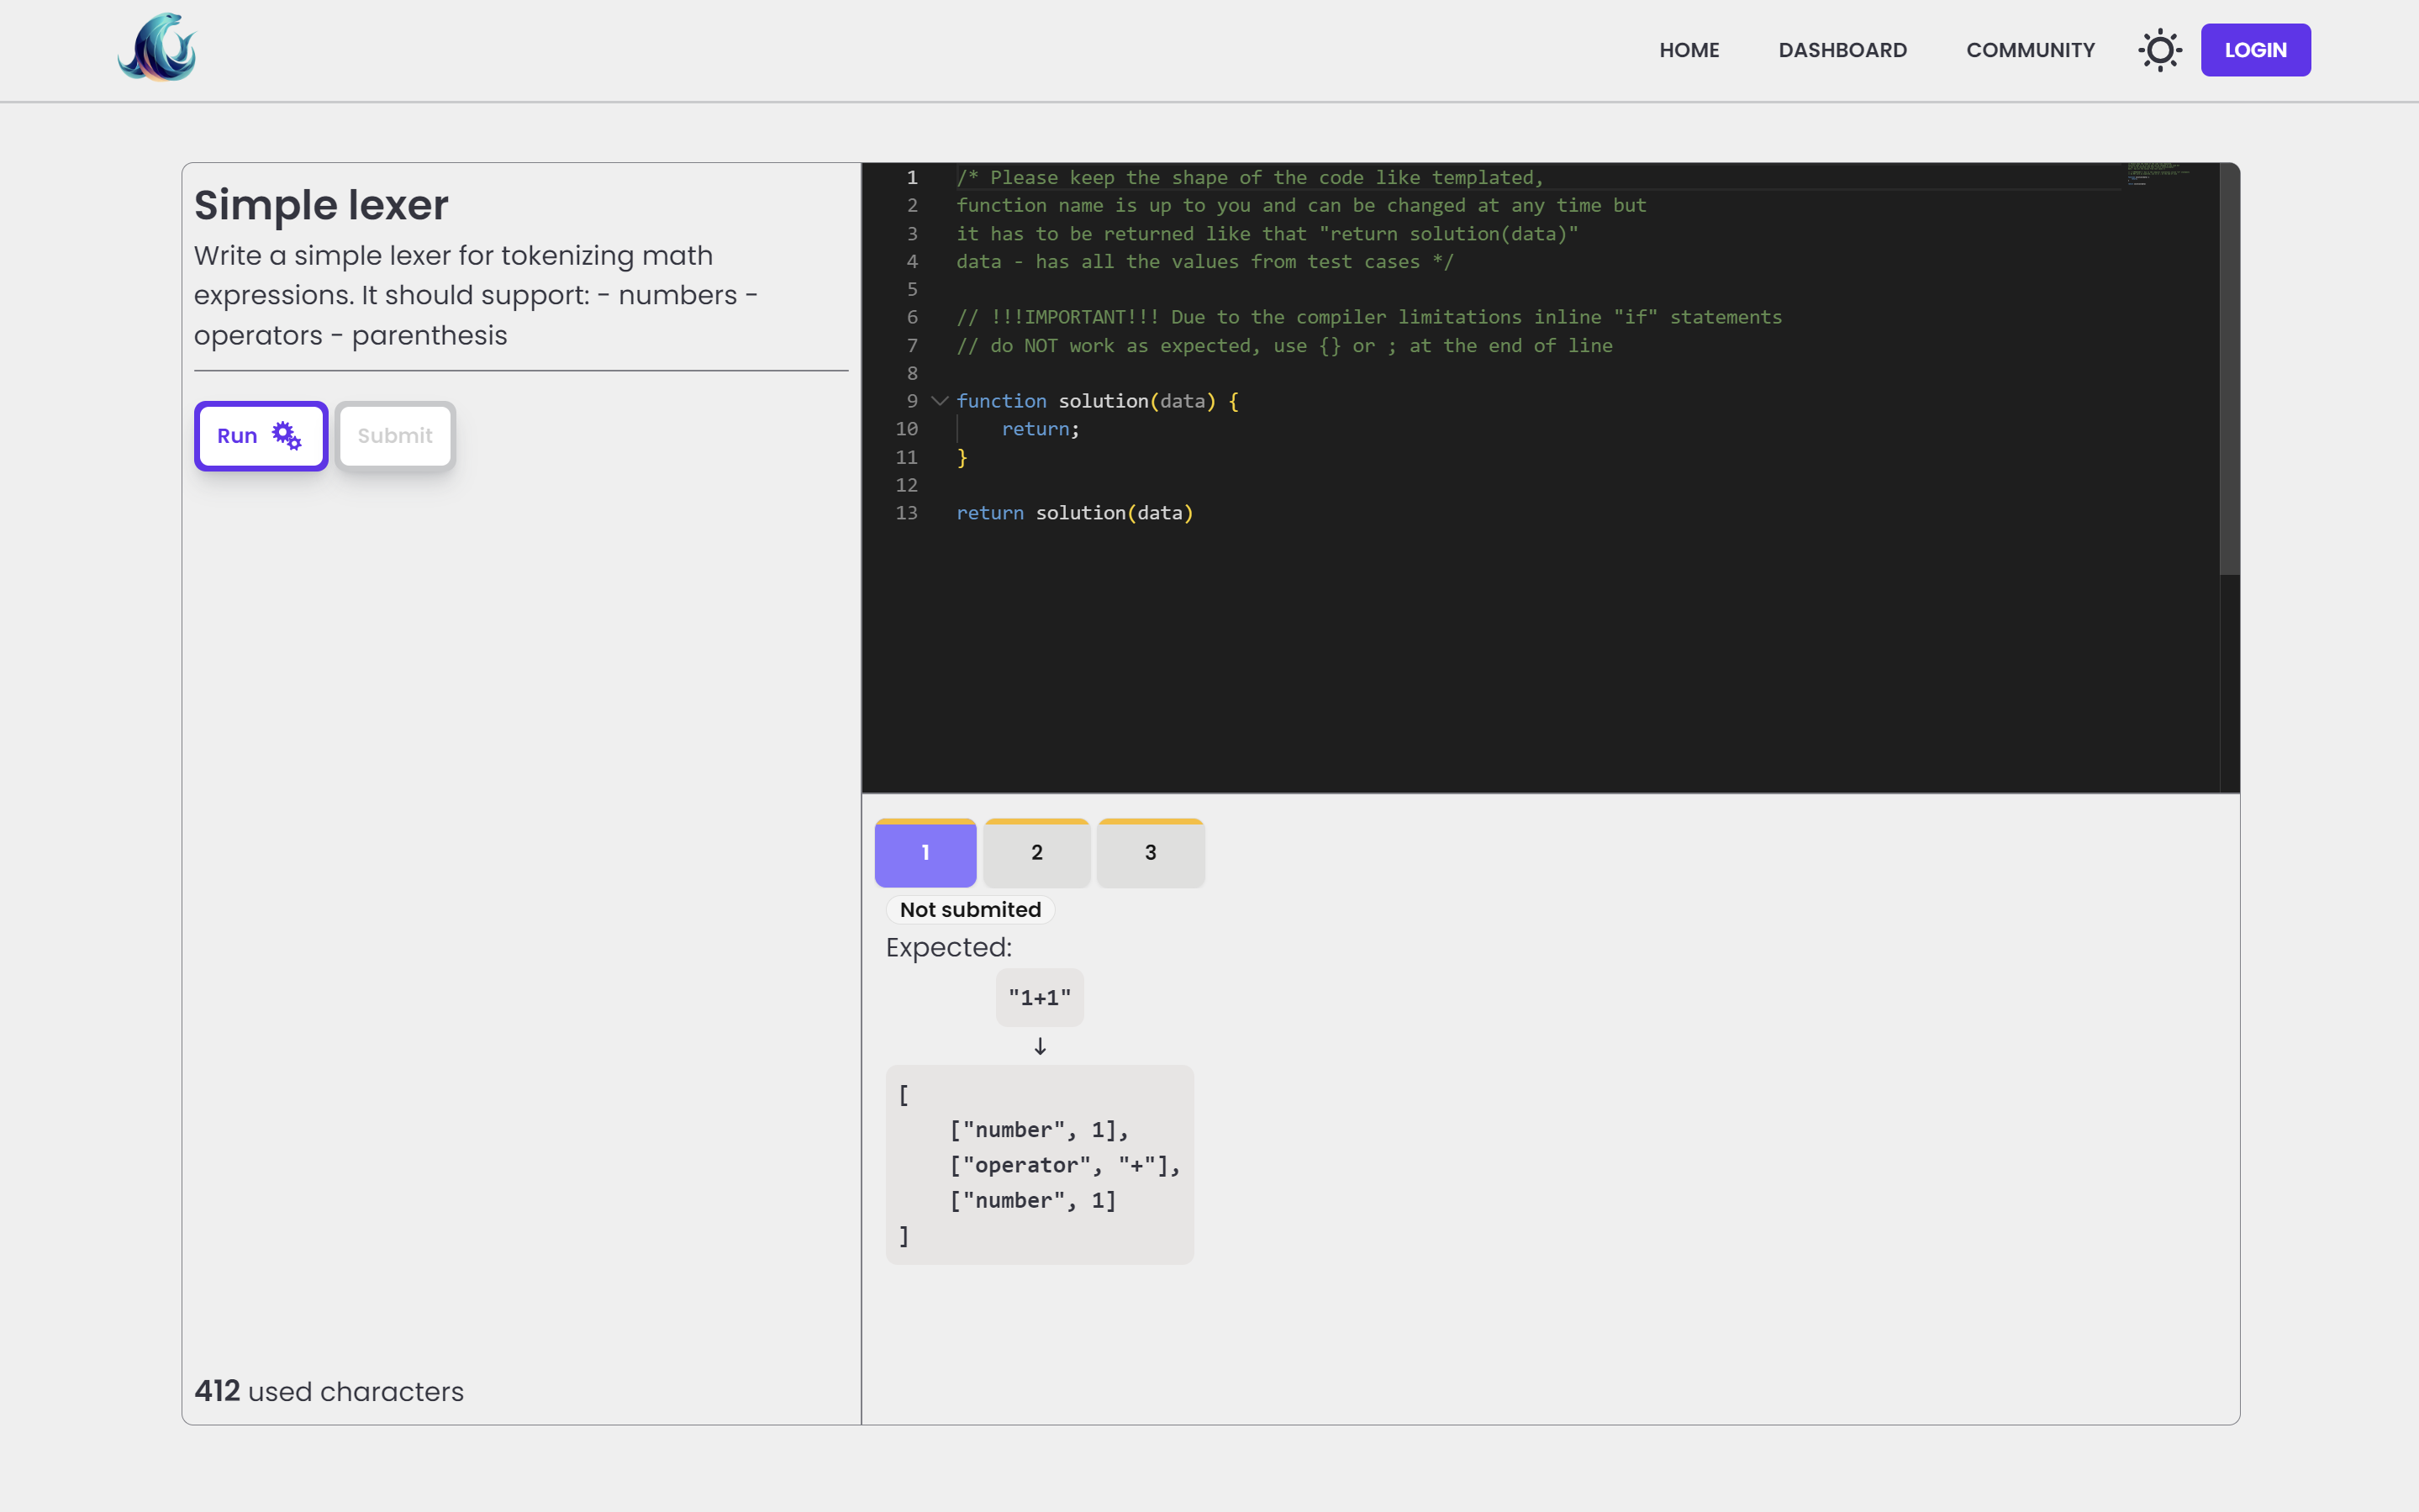
\includegraphics[width=0.75\linewidth]{image/programming.png} 
	\caption{Obrázek programovací úlohy.} %% popisek obrázku, nezapomeň na citace!
	\label{fig:programming} %% označení až budeš chtít na obrázek odkazovat
\end{figure}

\clearpage
\section{Zobrazování testů}

\subsection{Komunitní místo}
\label{subsec:community}
Na této stránce může uživatel objevit nové a populární testy, včetně všech dostupných testů. Testy se zobrazují postupně pomocí techniky \uv{infinite scrolling}, kde využívám JavaScript API Intersection Observer k~detekci, kdy uživatel dosáhl posledního prvku a následně si vyžádá další testy. Implementoval jsem vyhledávací pole, které umožňuje filtrovat zobrazené testy, a další možností je filtrace pomocí tagů. Vizuálně jsou testy rozlišeny mezi kvízy a programovacími úlohami. Uživatel může hodnotit testy hvězdičkou s~využitím principu \uv{optimistic update}. To znamená, že po přidání hvězdičky ji uživatel ihned vidí, přestože se zároveň ověřuje jeho oprávnění a vytváří se záznam hvězdičky v~databázi. V~případě neúspěchu se automaticky hvězdička odebere.

\begin{figure}[H]
	\centering %% příkaz, který ti obrázek zarovná na střed
	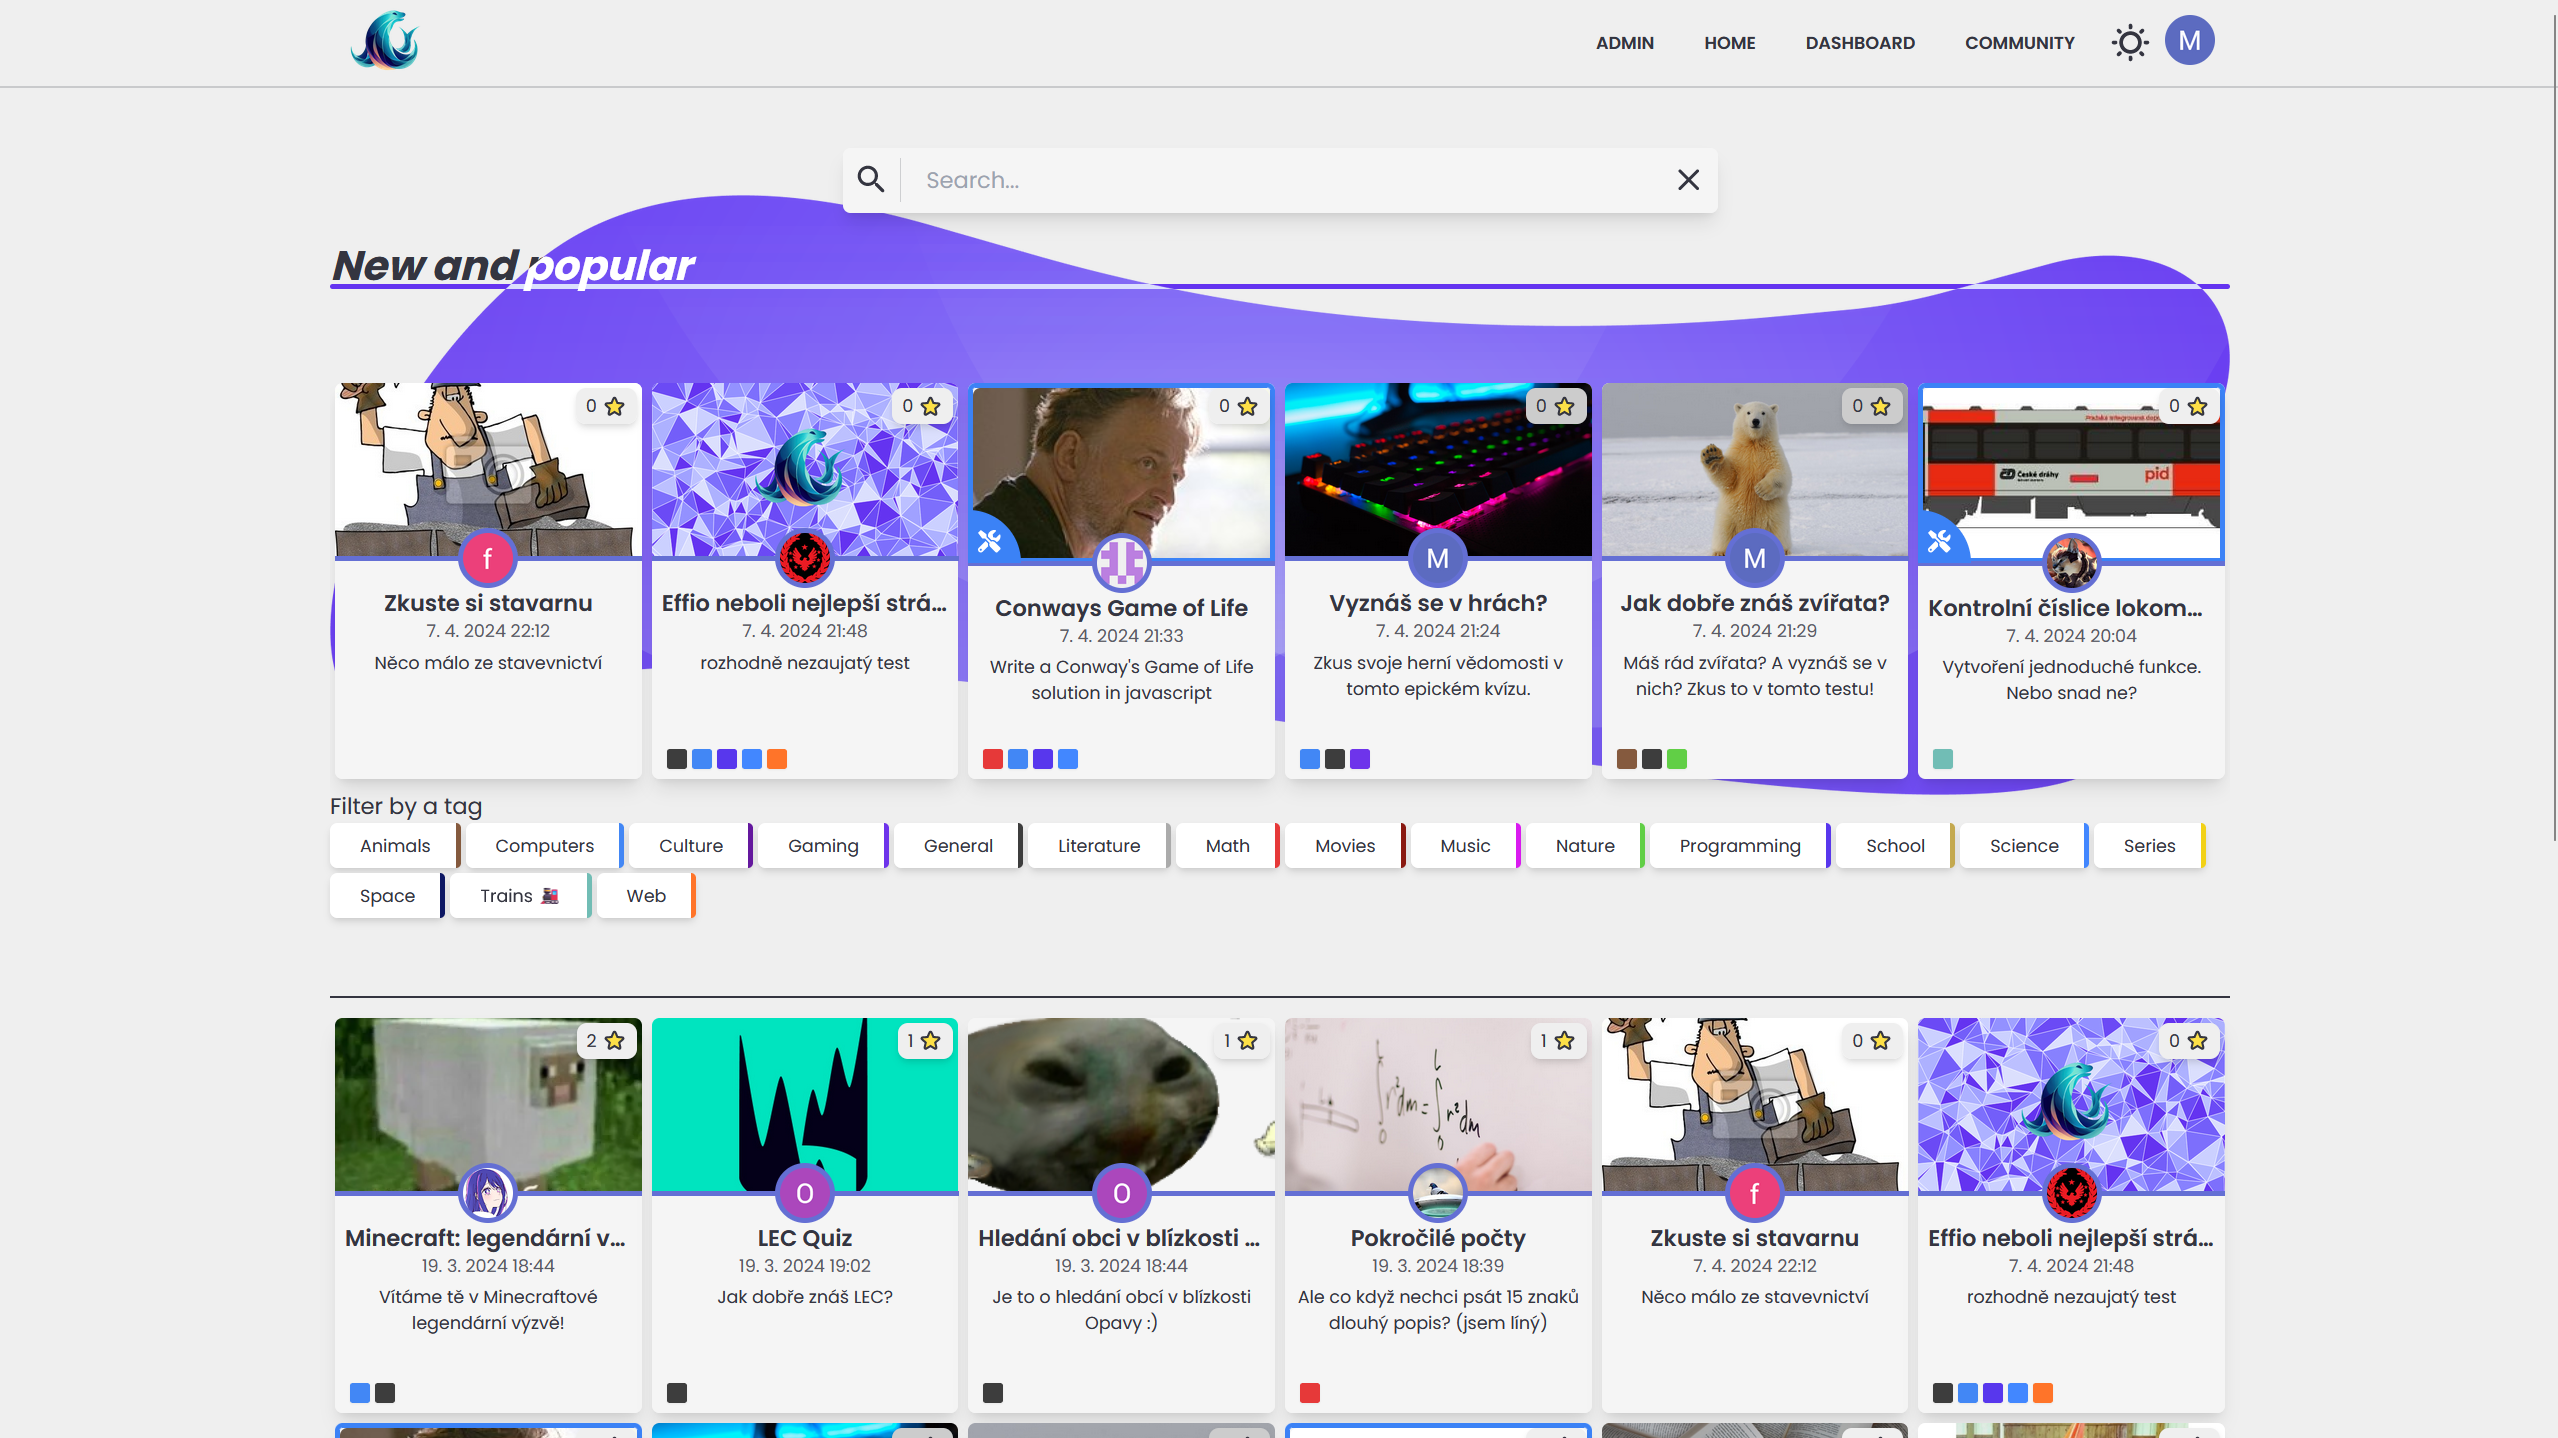
\includegraphics[width=1\linewidth]{image/community.png} 
	\caption{Komunitní místo.} %% popisek obrázku, nezapomeň na citace!
	\label{fig:community} %% označení až budeš chtít na obrázek odkazovat
\end{figure}


\subsection{Kolekce testů}
\label{subsec:collection}
Zde si uživatel může zobrazit jím vytvořené testy, aplikovaná je stejná funkcionalita vyhledávacího pole a \uv{infinite scrollingu}. Každý test má ale také další možnosti, a to úpravu, export a smazání.
\begin{itemize}
	\item Úprava - uživatel se přesune na stránku úprav, tam může celý test přepracovat.
	\item Export - vytvoří z~testu textový soubor ve formátu GIFT se všemi otázkami daného testu, které jsou podporovány Moodlem
	\item Delete - smazání testu z databáze
\end{itemize}

\subsection{Testová historie}
\label{subsec:historie}
Toto místo slouží pro zobrazení dříve vyplněných testů, na výpis testů je zde pro změnu využita metoda "pagination", která rozděluje jejich zobrazení na jednotlivé části, mezi kterými se přepíná. Na kliknutí na test se zobrazí záznam testu přesně v tom stavu jak ho uživatel dříve vyplnil.

\begin{figure}[H]
	\centering %% příkaz, který ti obrázek zarovná na střed
	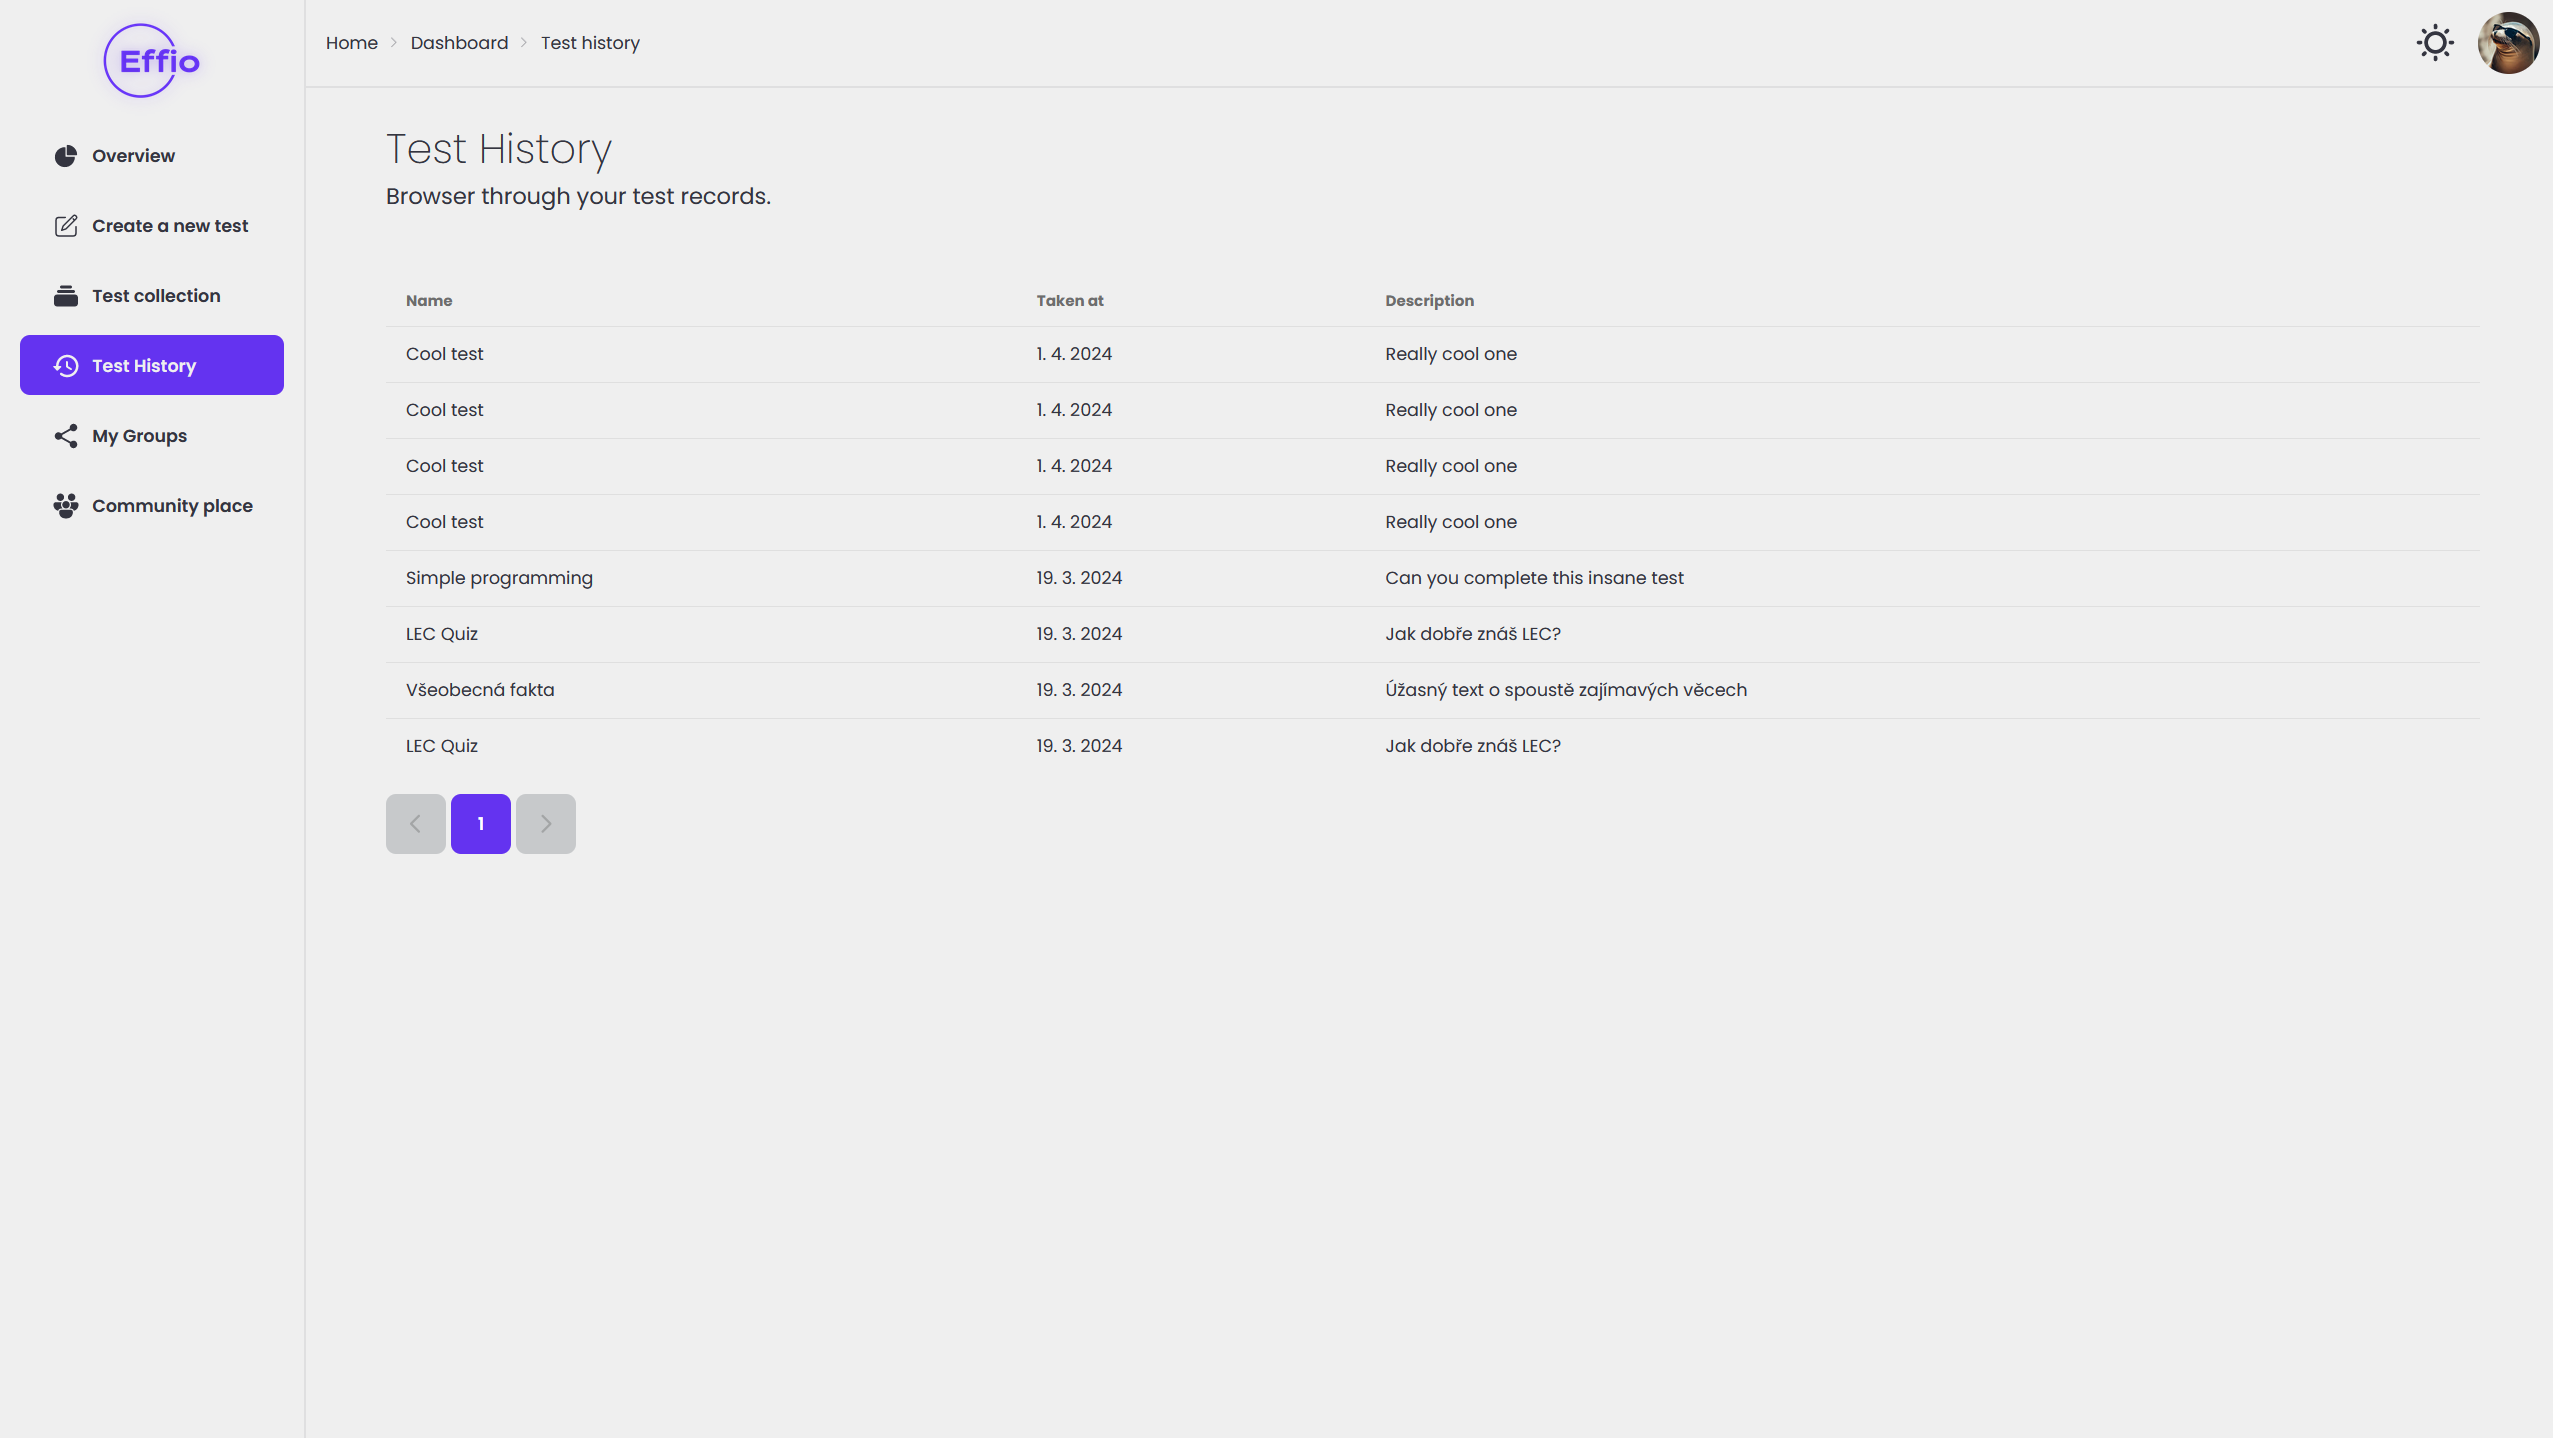
\includegraphics[width=1\linewidth]{image/history.png} 
	\caption{Testová historie} %% popisek obrázku, nezapomeň na citace!
	\label{fig:history} %% označení až budeš chtít na obrázek odkazovat
\end{figure}

\section{Skupiny}
Každý přihlášený uživatel si může vytvořit vlastní skupinu, do které se můžou pomocí generovaného kódu připojit ostatní uživatelé, tyto kódy se poté pomocí cronu mažou. Skupina obsahuje jednotlivé kanály, které funguje jednak jako chat (nebo pouze pro oznámení a psát do něj může pouze majitel), a také jako místo pro sdílení testů vlastníka, u těchto testů poté může vlastník kontrolovat vyplnění jednotlivými členy skupiny, grafy výsledků a také si zobrazit jednotlivá řešení uživatelů (na testy přidané do skupin lze aplikovat limit počtu vyplnění pro uživatele). Majitel má také možnost vyhodit/zabanovat jednotlivé členy.

\begin{figure}[H]
	\centering %% příkaz, který ti obrázek zarovná na střed
	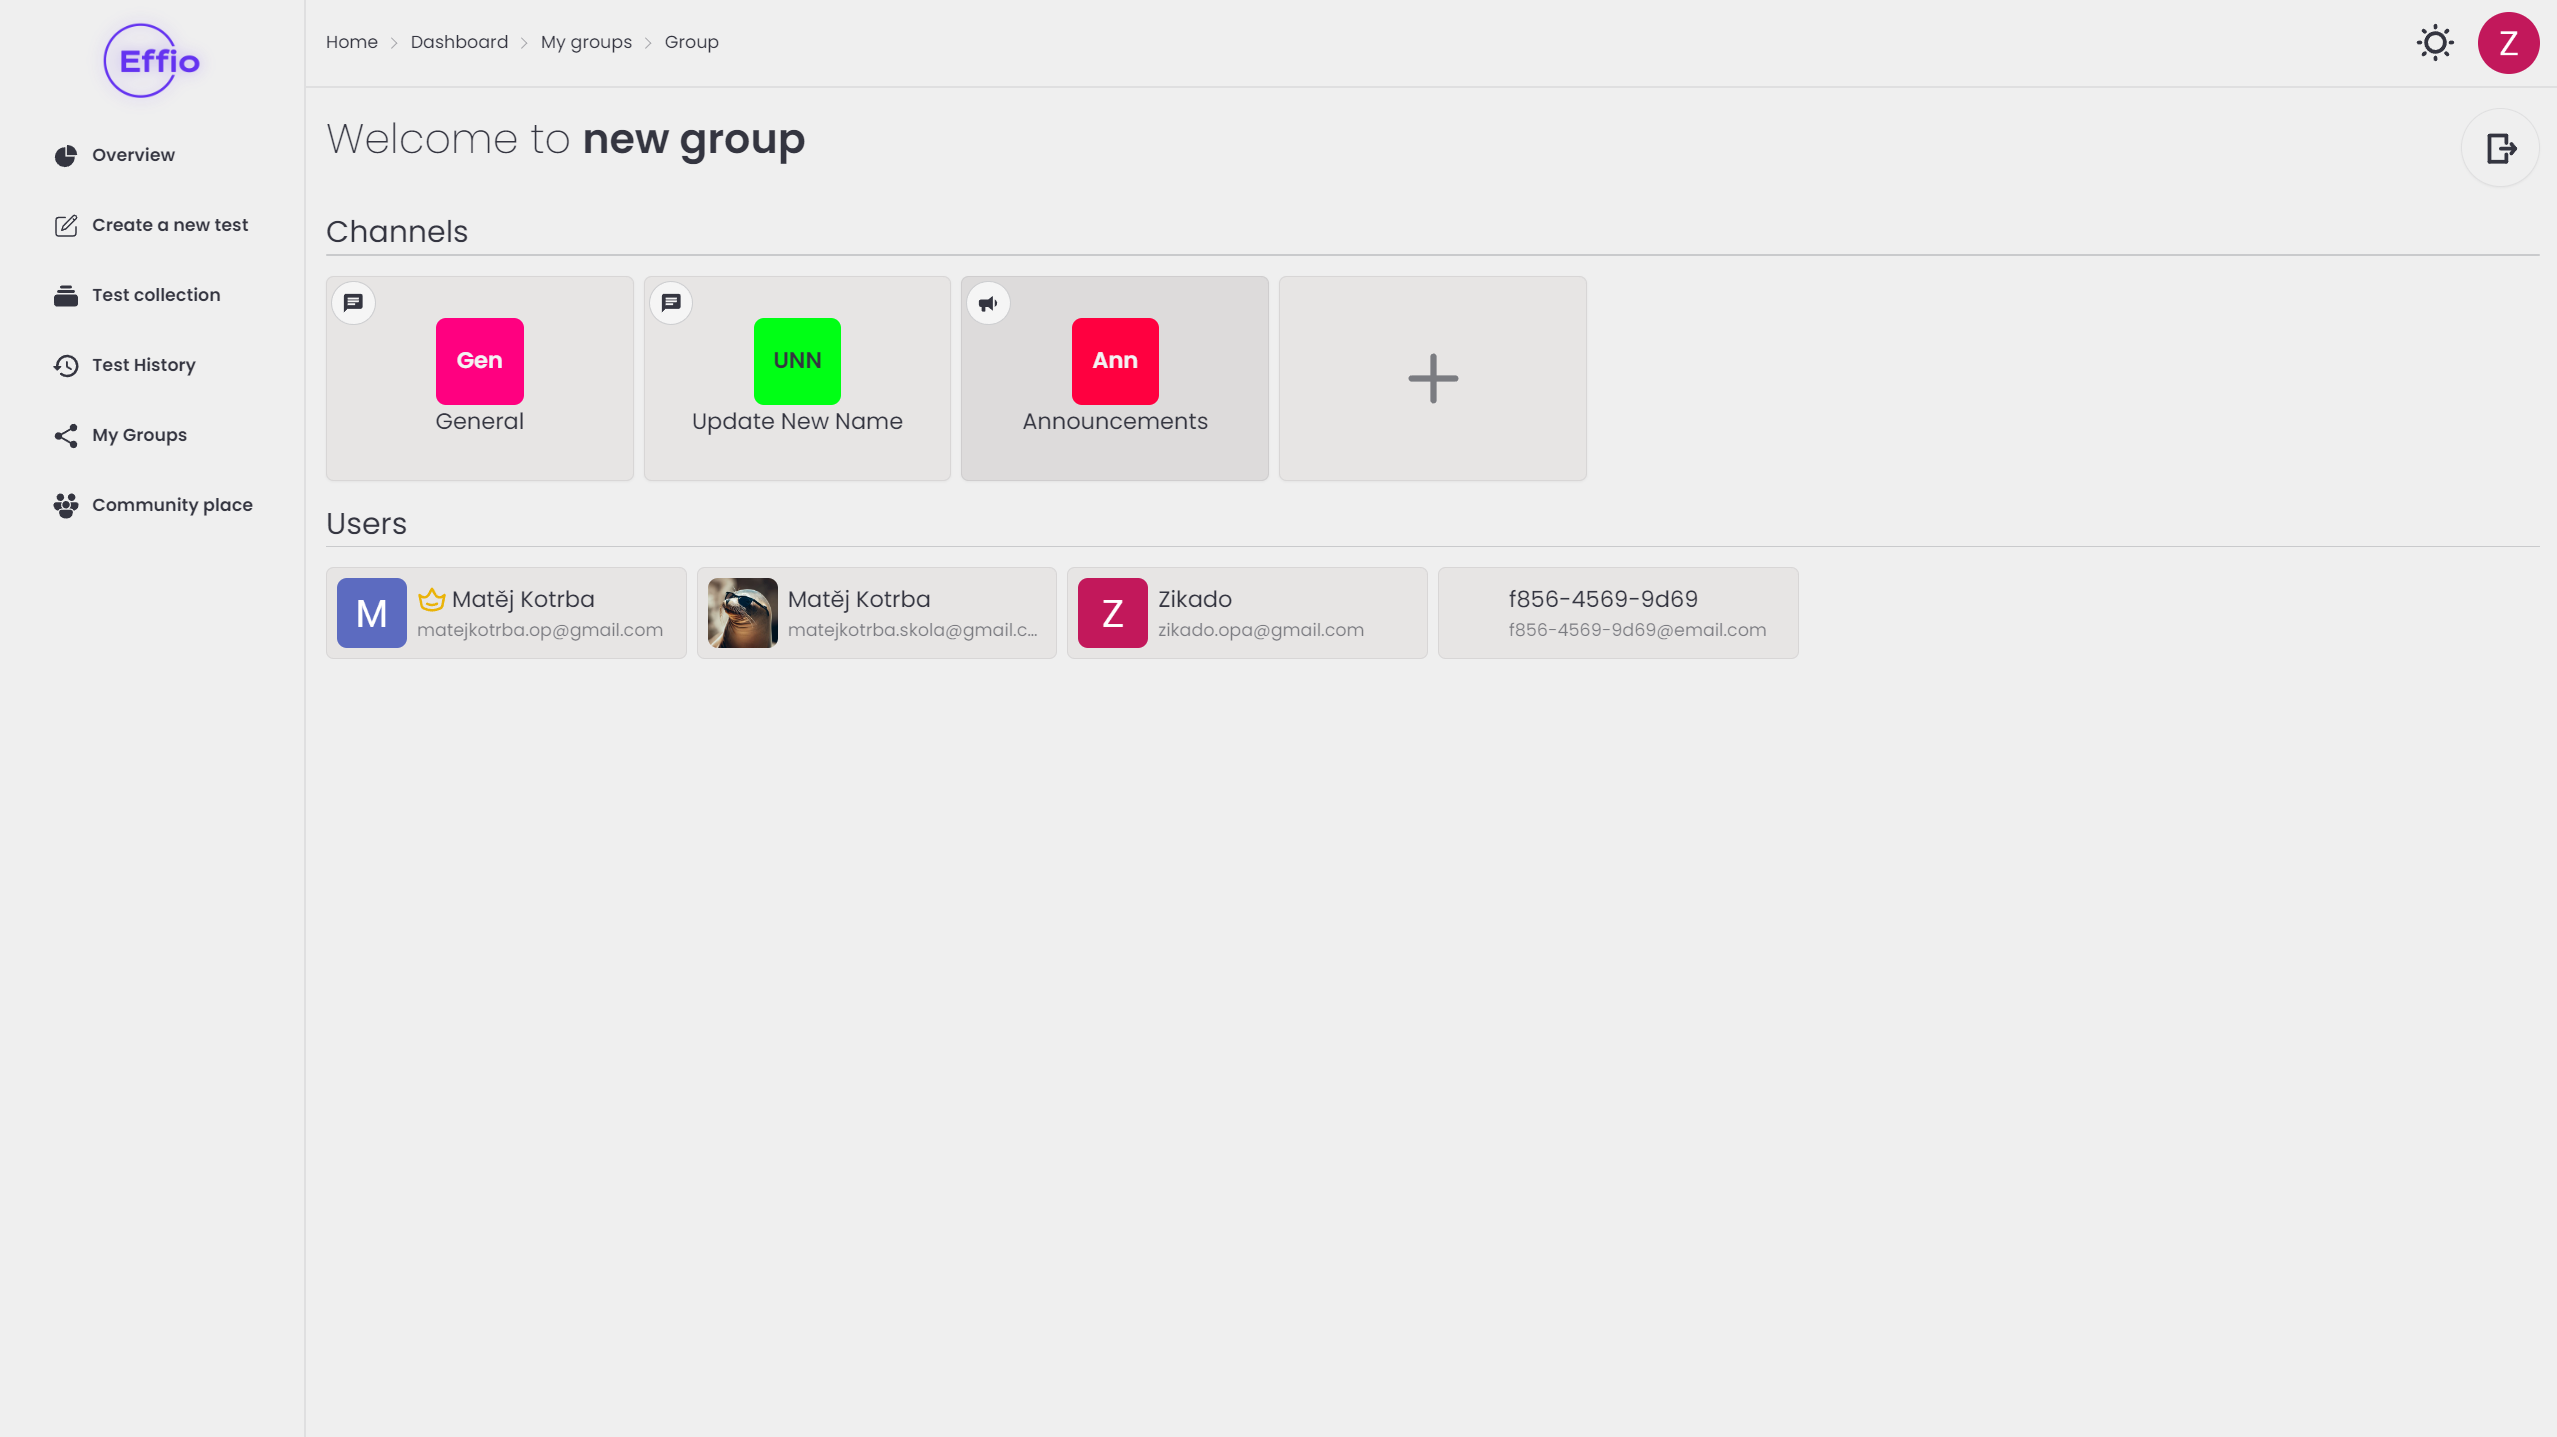
\includegraphics[width=1\linewidth]{image/groups.png} 
	\caption{Ukázka skupin} %% popisek obrázku, nezapomeň na citace!
	\label{fig:groups} %% označení až budeš chtít na obrázek odkazovat
\end{figure}

\section{Administrátorská část}
Pro administrátory aplikace je dostupná také stránka se správou jednotlivých testů a uživatelů, zde si je můžou zobrazit v tabulce a například je mazat nebo měnit uživatelské role. Další funkcí je také zobrazování logů akcií, které byli adminy provedeny.

\begin{figure}[H]
	\centering %% příkaz, který ti obrázek zarovná na střed
	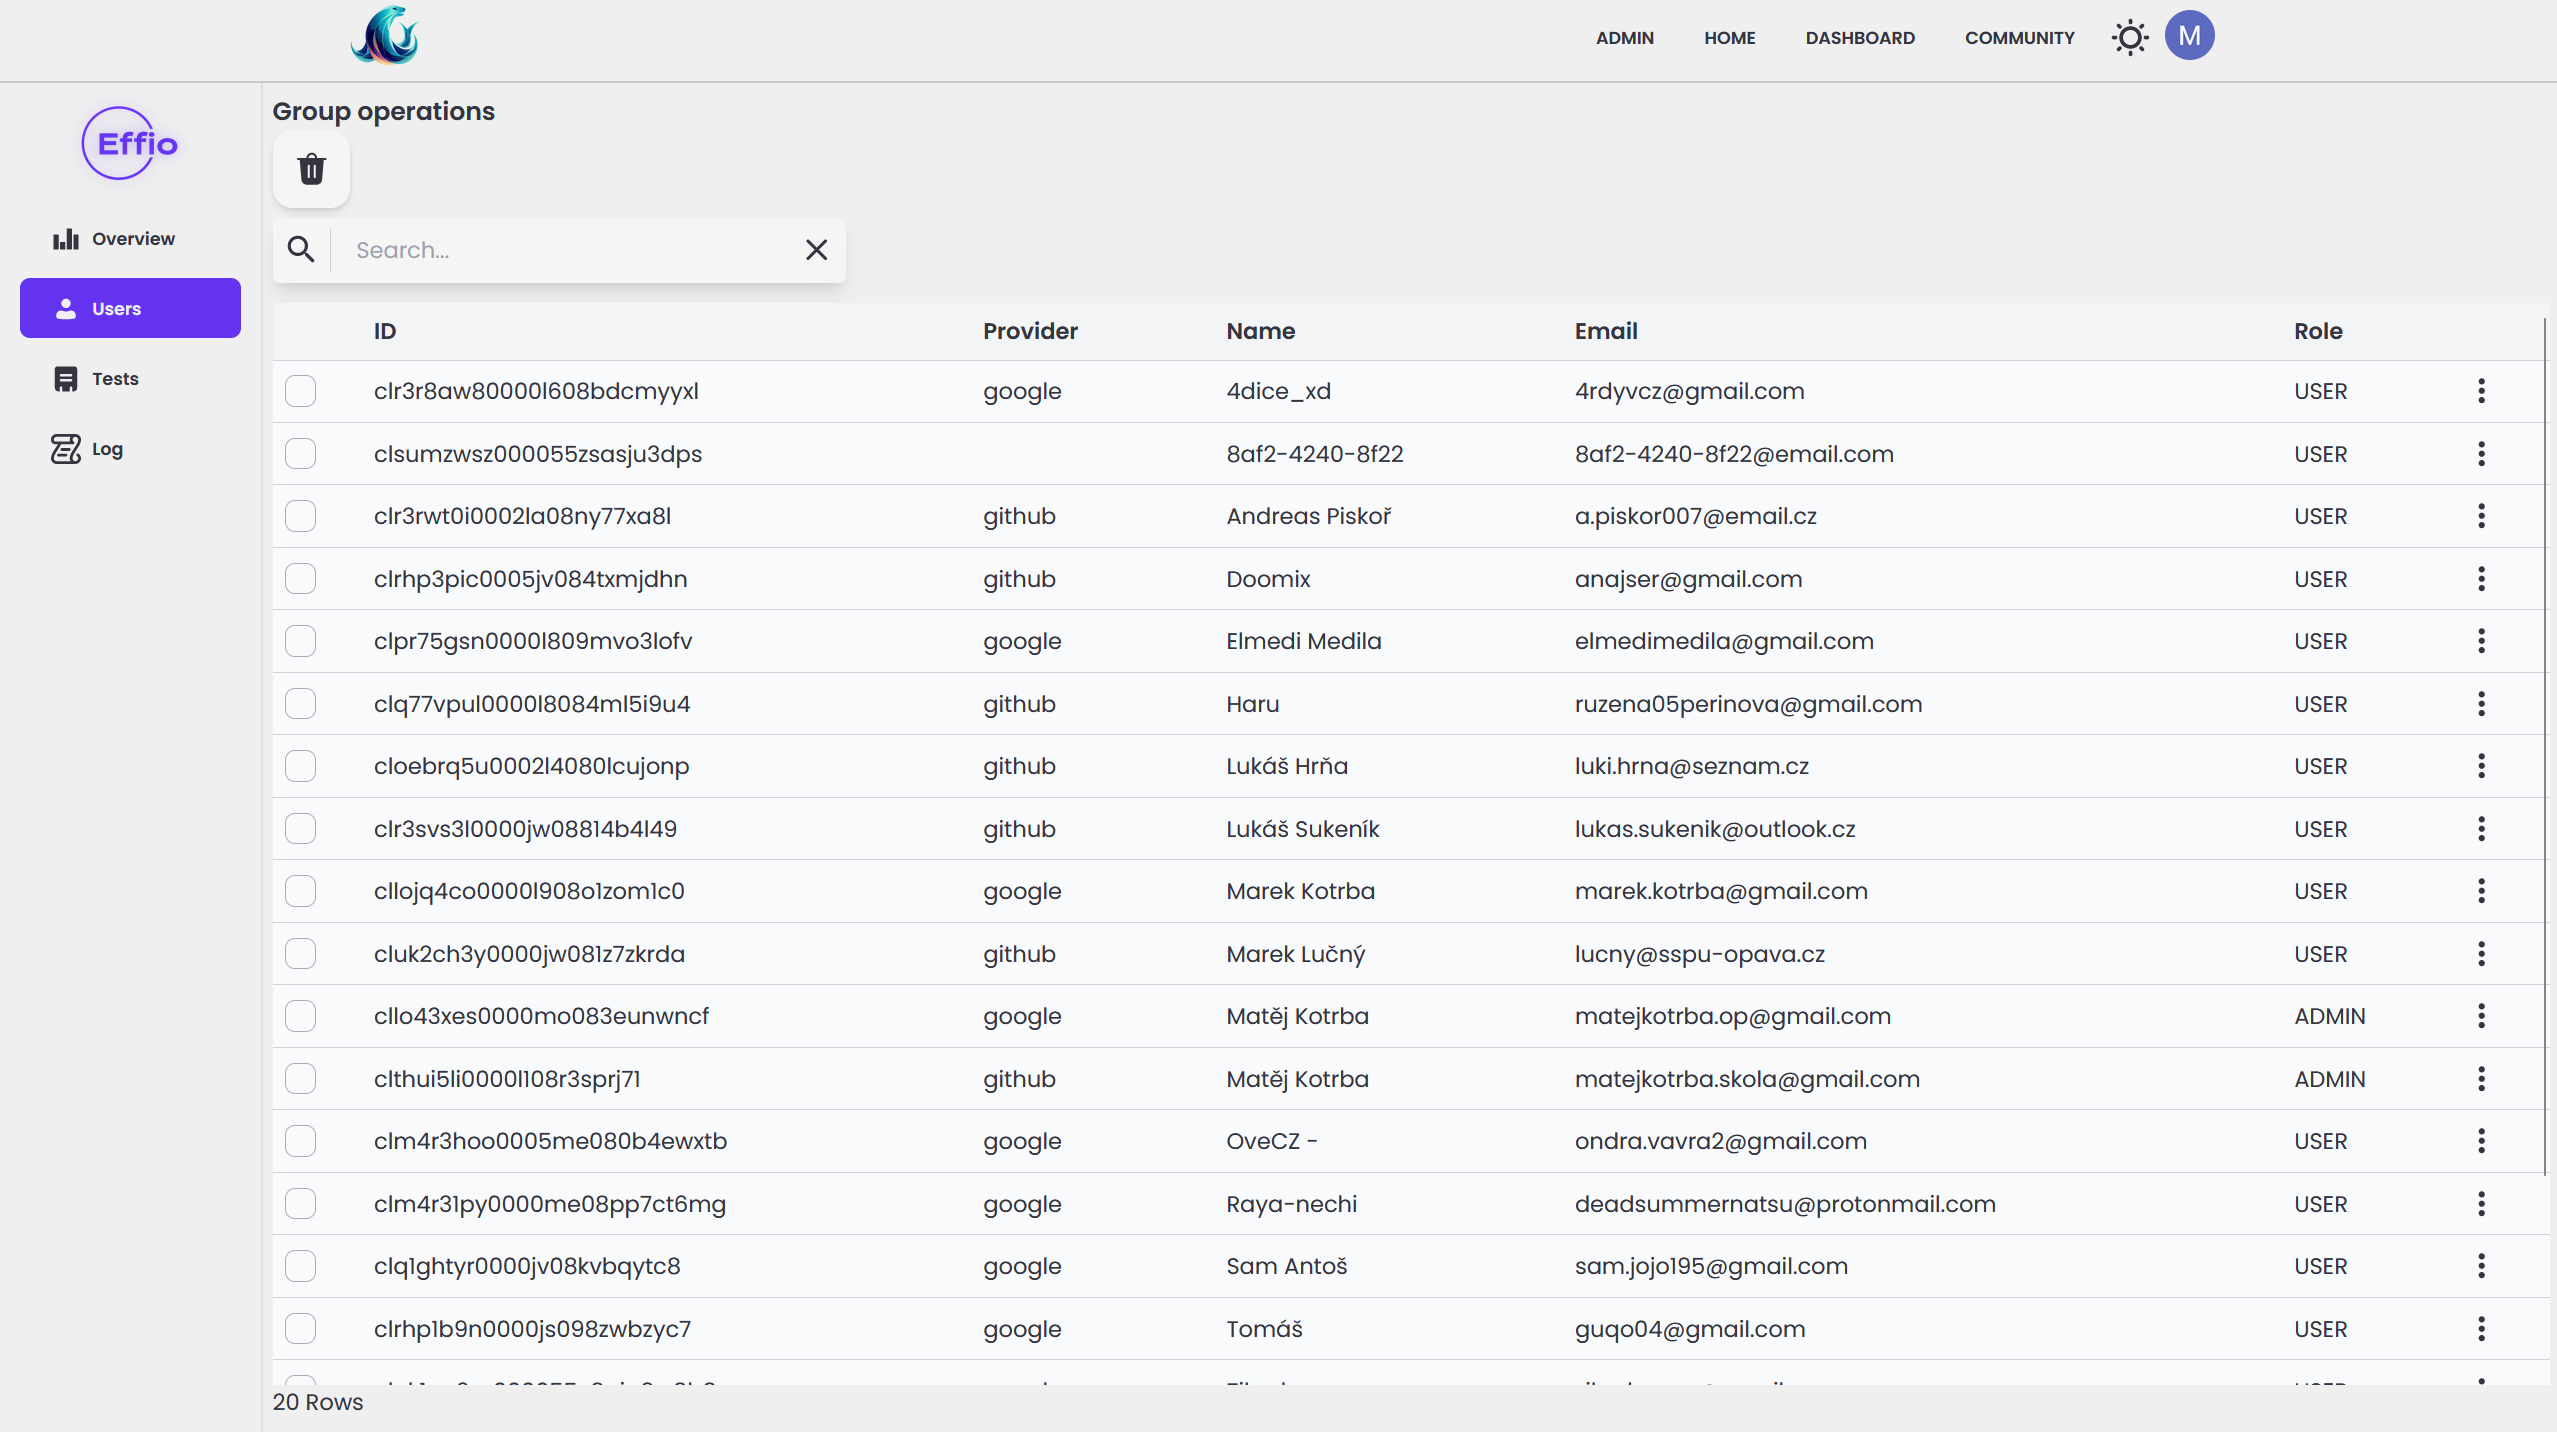
\includegraphics[width=1\linewidth]{image/admin.png} 
	\caption{Administrátorský panel} %% popisek obrázku, nezapomeň na citace!
	\label{fig:admin} %% označení až budeš chtít na obrázek odkazovat
\end{figure}

%\chapter{Výsledky práce}
%\section{Funkce aplikace}
%Po příchodu na stránku se uživateli zobrazí domovská stránka, zde může prozkoumat výhody aplikace nebo se přihlásit, to ho přesune na přihlašovací stránku, na ni se uživatel do aplikace může přihlásit pomocí Google nebo GitHub účtu. Po přihlášení je uživatel přesunut na dashboard, kde může vidět rychlou navigaci na další části nebo se podívat na souhrn jeho aktivity v~grafech. První možností je vytvořit si nový test, tato možnost je detailně probraná zde \ref{subsec:creation}.
%Po vytvoření testu je přesunut do kolekce jeho testů, kde může své testy procházet a upravovat, více popsáno zde \ref{subsec:collection}. Test si poté může uživatel zkusit vyplnit \ref{sec:test-take}, buď přímo ze své kolekce nebo z komunitního centra \ref{subsec:community}, kde může najít také testy jiných. Po dokončení testu se dozví výsledky, ty může poté najít zpětně v~sekci \textit{Test history}, kde jsou uspořádané v tabulce.

\chapter{Zhodnocení práce}

\section{Splněné a nesplněné cíle}
Hlavním cílem bylo vytvořit rychlou, cloudovou aplikaci pro vytváření a sdílení testů využívající moderních \uv{techstack}, v~tomto ohledu jsem cíl kompletně splnil, aplikace je v~těchto bodech plně funkční a můj původní plán využití technologií se během vývoje ještě významně rozrostl. Aplikace mimo již výše zmíněné možnosti nabízí také historii, export a import, skupiny, administrátorskou část a spoustu menších dílčích prvků dotvářející celkový dojem.

Za úspěch považuji také grafickou část aplikace, která za mě tvoří minimalistický moderní vzhled, responsivitu umožňující využití aplikace na více zařízení a barevně vyvážený světlý a tmavý režim.

\section{Produkční připravenost}
Díky zvoleným technologiím si dovoluji aplikaci prohlásit za produkčně způsobilou, jednotlivé služby mají snadnou možnost škálování, implementace je z~velké většiny stabilní.

Možnosti využití aplikace jsou od nenáročného občasného návštěvníka, který si chce zkusit nějaký kvíz, až po implementaci v~rámci třídy, kde učitel zadá kvíz, který následně žáci musejí vyplnit.

\section{Možná vylepšení}
Nelze ale říct, že by aplikace byla dokonalá, určitě je zde prostor pro mnoha vylepšení v~rámci funkcionality, ať už jde o například přidání časového limitu do kvízů, více individuálních funkcí pro členy skupiny nebo třeba širší možnosti sociálního rázu, jako třeba zobrazování profilu apod.

\chapter*{Závěr}
	
Cílem projektu bylo vytvořit webovou aplikaci pro vytváření a vyplňování testů. Aplikace je postavená na frameworku SvelteKit, psaný v~jazyce TypeScript. Přihlašování stojí na knihovně Auth.js, MySQL databáze je hostovaná službou Planetscale, jako ORM je použita Prisma. Frontend řeší framework Svelte s~CSS utility knihovnou Tailwind, pro validaci využívá Zod.

Základem aplikace je generátor testů, kde uživatel využívá předpřipravené typy otázek. Testy se následně dají vyplnit v~rámci komunity nebo vlastníkovi kolekce. Nepřihlášený uživatel může testy pouze vyplňovat, přihlásit se uživatel může pomocí Google nebo GitHub účtu. Uživatelé také mají k~dispozici skupiny kde je chat a také možnosti sdílet testy společně s výsledky a grafy pro vlastníka, test historii k~zobrazení dříve vyplněných testů a přehled nedávné aktivity v~podobě grafů. Využité technologie činí aplikaci lehce škálovatelnou a velice výkonnou. Aplikace je téměř zcela funkční a použitelná na všech zařízeních díky responzivnímu designu.

\noindent Aplikace je zálohovaná na GitHubu na adrese \url{https://github.com/matej-kotrba/effio}.
Je také volně přístupná na adrese \url{https://effio.vercel.app/}
	
	%% literatura
	\renewcommand\bibname{Seznam použitých informačních zdrojů}
	\begin{thebibliography}{99}
		
		\bibitem{Svelte} Svelte [online]. 2023 [cit. 2023-12-27]. Dostupné z: \url{https://svelte.dev/}
		\bibitem{SvelteKit} SvelteKit [online]. 2023 [cit. 2023-12-27]. Dostupné z:  \url{https://kit.svelte.dev/}
		\bibitem{tRPC} tRPC [online]. 2023 [cit. 2023-12-27]. Dostupné z: \url{https://trpc.io/}
		\bibitem{Prisma} Prisma [online]. 2023 [cit. 2023-12-27]. Dostupné z: \url{https://www.prisma.io/}
		\bibitem{Zod} Zod [online]. 2023 [cit. 2023-12-27]. Dostupné z: \url{https://zod.dev/}
		\bibitem{Auth.js} Auth.js [online]. 2023 [cit. 2023-12-27]. Dostupné z: \url{https://authjs.dev/}
		\bibitem{Tailwind CSS} Tailwind CSS [online]. 2023 [cit. 2023-12-27]. Dostupné z: \url{https://tailwindcss.com/}
		\bibitem{tRPC-SvelteKit} tRPC-SvelteKit [online]. 2023 [cit. 2023-12-27]. Dostupné z: \url{https://icflorescu.github.io/trpc-sveltekit/}
		\bibitem{ChatGPT} ChatGPT [online]. 2023 [cit. 2023-12-27]. Dostupné z: \url{https://chat.openai.com/}
		\bibitem{Stackoverflow} Stackoverflow [online]. 2023 [cit. 2023-12-27]. Dostupné z: \url{https://stackoverflow.com/}
		\bibitem{Joy of Code}Joy of Code. Youtube kanál. Https://www.youtube.com/ [online]. 2023 [cit. 2023-12-27]. Dostupné z: \url{https://www.youtube.com/@JoyofCodeDev}
		\bibitem{Huntabyte}Huntabyte. Youtube kanál. Https://www.youtube.com/ [online]. 2023 [cit. 2023-12-27]. Dostupné z: \url{https://www.youtube.com/@Huntabyte}
		\bibitem{Theo}BROWNE, Theo. Youtube kanál. Https://www.youtube.com/ [online]. 2023 [cit. 2023-12-27]. Dostupné z: \url{https://www.youtube.com/@t3dotgg}
		\bibitem{Kevin Powell}POWELL, Kevin. Youtube kanál. Https://www.youtube.com/ [online]. 2023 [cit. 2023-12-27]. Dostupné z: \url{https://www.youtube.com/@KevinPowell}
		\
		
	\end{thebibliography}
	
	%% obrázky 
	\listoffigures
	

	\appendix %% začínají přílohy
	
	\titleformat{\chapter}[block]{\scshape\bfseries\LARGE}{Příloha \thechapter}{10pt}{\vspace{0pt}}[\vspace{-22pt}] %% nastavení nadpisu u příloh

	\chapter{Databázový model}

	\begin{figure}[H]
		\centering %% příkaz, který ti obrázek zarovná na střed
		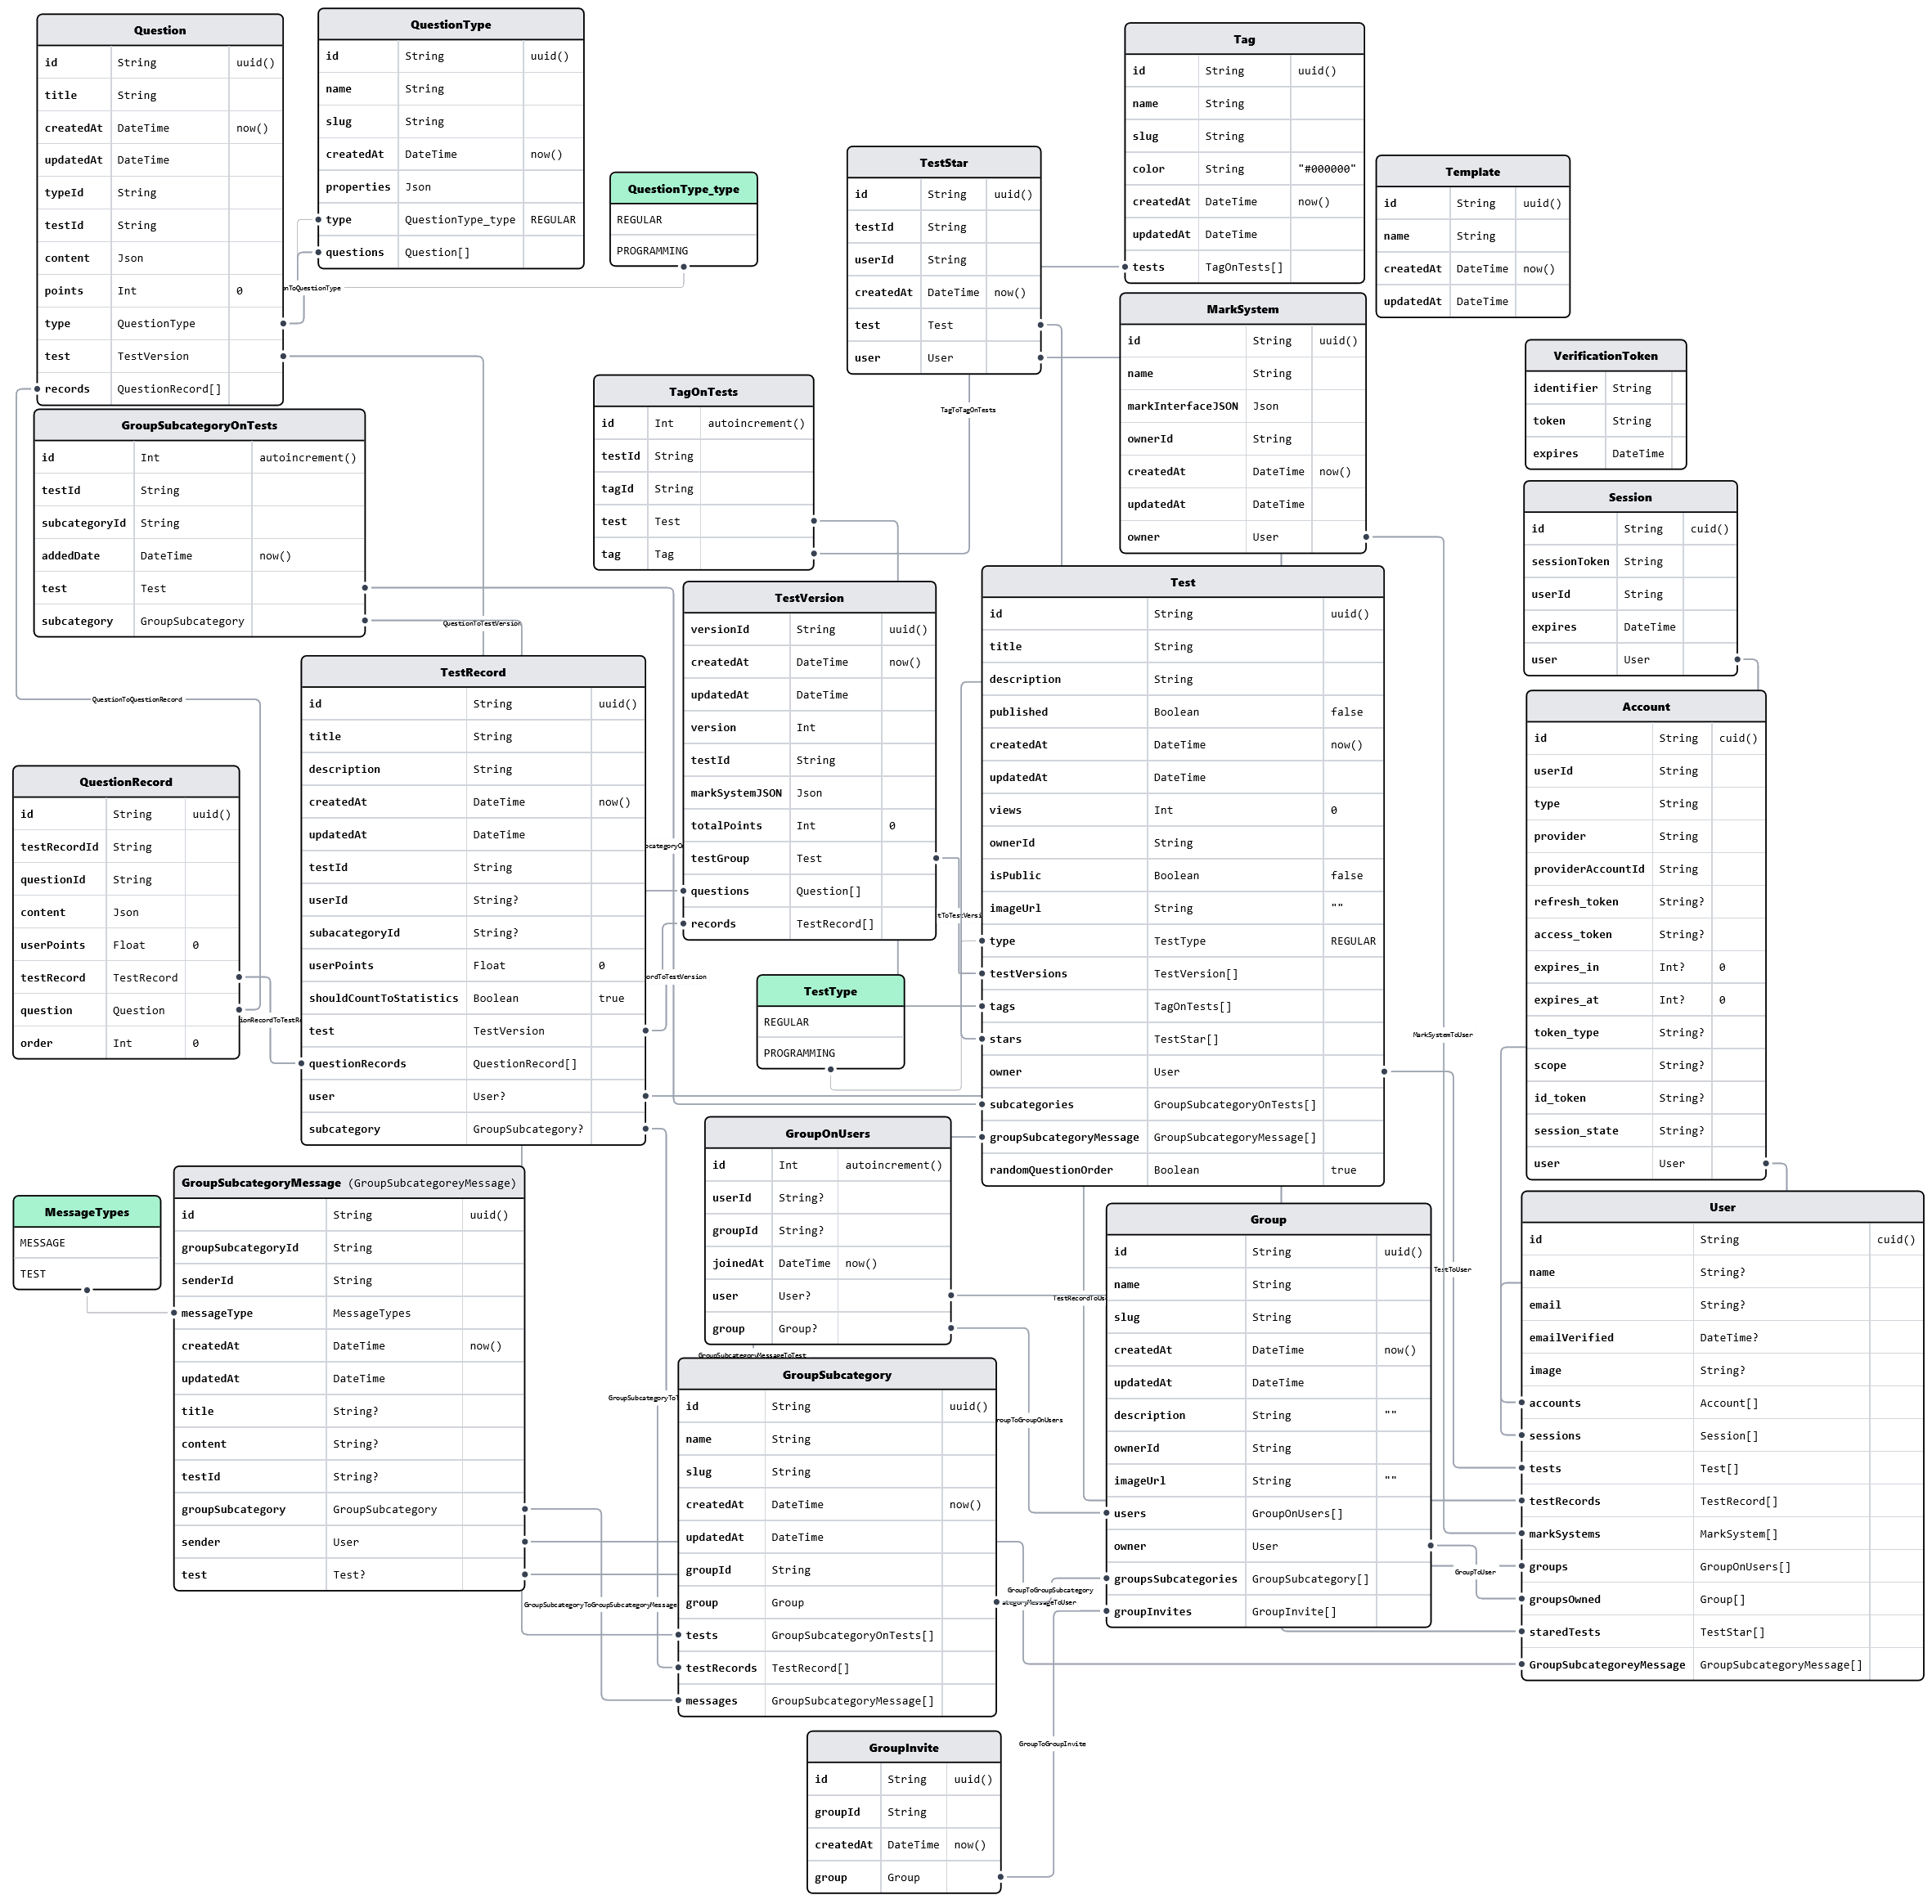
\includegraphics[width=0.9\linewidth]{image/schema.png} 
		\caption{Databázový model Effia. Vytvořeno pomocí \href{https://github.com/Ovyerus/prismaliser}{Prismaliser}} %% popisek obrázku, nezapomeň na citace!
		\label{fig:schema} %% označení až budeš chtít na obrázek odkazovat
	\end{figure}
	
\end{document}